\documentclass[a4paper, english]{article}

% includes 
% Language setting
\usepackage[english]{babel}
\usepackage{csquotes}
\usepackage[iso]{isodate}
\usepackage[version=4]{mhchem} % for chemical reaction formulas
% Set page size and margins
\usepackage[top=2cm,bottom=2cm,left=3cm,right=3cm,marginparwidth=1.75cm]{geometry}
%% images
\usepackage{graphicx}
\usepackage{wrapfig}
\usepackage[inkscapeformat=png]{svg}
%% captions 
\usepackage{caption}
\usepackage{subcaption}
%% tables 
\usepackage{booktabs}
%% colors
\usepackage{xcolor}
%% links and refs and citations 
\usepackage{setspace}
\usepackage[colorlinks=true, allcolors=blue]{hyperref}
\usepackage[capitalize]{cleveref}
\usepackage[backend=biber, style=authoryear]{biblatex}
%% acronyms and glossary 
%\usepackage[acronym,]{glossaries} 
\usepackage[automake,acronym,postdot,stylemods,translate=babel]{glossaries-extra}
%% include code snippets
\usepackage{listings}
%% Kerning
\usepackage[protrusion=true,expansion]{microtype}
%% maths
\usepackage{amsmath}
%% Tikz
\usepackage{tikz}
\usetikzlibrary{shapes.geometric, arrows}
%% Some diagram definitions
  %
\tikzstyle{startstop} = [rectangle, rounded corners, minimum width=3cm, minimum height=1cm,text centered, draw=black, fill=red!30]
\tikzstyle{io} = [trapezium, trapezium left angle=70, trapezium right angle=110, minimum width=3cm, minimum height=1cm, text centered, draw=black, fill=blue!30]
\tikzstyle{process} = [rectangle, minimum width=3cm, minimum height=1cm, text centered, draw=black, fill=orange!30]
\tikzstyle{decision} = [diamond, minimum width=3cm, minimum height=1cm, text centered, draw=black, fill=green!30]
\tikzstyle{arrow} = [thick,->,>=stealth]

%% title page
\usepackage{titling} % for cooler titlepages 
% configuration 
\bibliography{refs.bib} % Entries are in the refs.bib file
% configure python code snippets
\lstdefinestyle{PyStyle}{%
    commentstyle=\color{olive},
    keywordstyle=\color{magenta},
    numberstyle=\tiny\color{gray},
    stringstyle=\color{purple},
    basicstyle=\footnotesize,
    breakatwhitespace=false,         
    breaklines=true,                 
    captionpos=b,                    
    keepspaces=true,                 
    numbers=left,                    
    numbersep=5pt,                  
    showspaces=false,                
    showstringspaces=false,
    showtabs=false,                  
    tabsize=2,
    language=python
}
% setup title 
\title{\textbf{\huge Impact of Climate and Land Cover Change in Urban Heat Islands} }
\author{Linus Andrae (6015384)}
\date{\today}

\makeglossaries%
\setabbreviationstyle[acronym]{long-short}
% Acros
\newacronym{USGS} {USGS} {United States Geological Survey}
\newacronym{LST}  {LST}  {Land Surface Temperature}
\newacronym{LULC} {LULC} {Land Use/ Land Cover}
\newacronym{UHI}  {UHI}  {Urban Heat Island}
\newacronym{SUHI} {SUHI} {Surface Urban Heat Island}
\newacronym{NDVI} {NDVI} {Normalized Differential Vegetation Index}
\newacronym{HI}   {HI}   {Heat Index}
\newacronym{NIR}  {NIR}  {Near Infrared}
\newacronym{OSM}  {OSM}  {Open Street Map}
\newacronym{TOA}  {TOA}  {Top of Atmosphere}
\newacronym{VOC}  {VOC}  {Volatile Organic Compounds}
\newacronym{ML}   {ML}   {Machine Learning}
\newacronym{SVM}  {SVM}  {Support Vector Machine}
\newacronym{ECMWF}{ECMWF}{European Center for Medium-Range Weather Forcasts}
\newacronym{WBGT} {WBGT} {Wet Bulb Globe Temperature}


\newglossaryentry{lib}%
{%
  name={library},
  description={a bundled collection of resources (e.g. algorithm) to be ease software development}
}

\newglossaryentry{sentinel3}%
{%
  name={Sentinel-3},
  description={A Pair of Satellites, that are part of the Copernicus constellation. Using 21 spectral channels with a resolution of 300~m per pixel}
}
\begin{document}
  \begin{titlingpage} %This starts the title page
\pagenumbering{Alph}
\thispagestyle{empty} 
\begin{center}
\begin{large}
  \textit{University Bremen}\\
\end{large}
\vspace{4cm} %You can control the vertical distance
\begin{large} 
\textbf{\thetitle} 
\end{large}
\theauthor\\
\thedate\\
\vspace{13cm} %Put the distance you need.


\includegraphics[width=0.3\textwidth]{img/res/uniLogoIUP.png}
\hspace{4cm}

\includegraphics[width=0.3\textwidth]{img/res/logo_ohb_digital.png}

\end{center}
\end{titlingpage}
\pagenumbering{arabic}

  \singlespacing%
  \newpage

  \begin{abstract}
\noindent
Urban Heat Islands (\acp{UHI}) pose a growing health risk by exacerbating heat stress for residents of urban areas. 
Due to the increased prevalence of extreme weather events and heat waves and as a cause for higher energy consumption, \acp{UHI} become more relevant as a topic for city planners and policy makers to consider.
Identification of areas most impacted or at risk require a data backed tool set to aid urban planning. 
This study presents a comprehensive pipeline developed using Python to automate the processing and analysis of Landsat 7,8 and 9 remote sensing imagery.
The pipeline facilitates the generation of Normalized Difference Vegetation Index (NDVI) and heat maps, running statistical analysis of factors known to create \acp{UHI} of a provided area of interest, serving as a robust toolset for the investigation and detection of \acp{UHI}.
The methodology employed leverages the spectral characteristics of Landsat data to provide high-resolution insights into temperature variations within urban areas as well as statistical analysis of the composition of the identified Urban Heat Islands.
The ultimate aim is to offer actionable guidance to city planners and developers for the mitigation of \acp{UHI}, by classification of \acp{UHI} on different scales.
At the current implementation level the pipeline is able to detect \acp{UHI} from level one brightness temperature and the statistical analysis indicate a strong correlation between land cover types and heat island intensity, affirming the utility of the pipeline in urban climate studies.
%To analyse and identify Urban Heat Islands using remote sensing imagery
\end{abstract}

  \newpage
  % TODO insert Eigenständigkeitserklärung

  \tableofcontents
  \listoffigures
  \listoftables
  \newpage
  % Abbreviations first
  %\printglossary[title=Abbreviations, type=abbreviations]
  \printglossary[title=Acronyms, type=acronym]
  %then the main glossary
  \printglossary%
\newpage

\section{A historical introduction of urban heat island research}
  The scientific investigation of the urban climate and the influence of human settlements and activity on the local atmosphere and temperature has been studied for more then 200 years.%
  \cite{Howard1833}~investigated the climate of London in a study from 1819 to 1827 and a similar study was conducted in Paris in the 1850s by~\cite{renou1862differences}.%
  The first mobile measurement campaigns by~\cite{peppler1929auto} and investigations of the spacial distribution of temperatures where conducted in the 1920s in Germany and Austria~\cite{tollner1932untersuchungen}, and where repeated in multiple cities around the globe.\\%todo add more refs? 
  The term Urban Heat Island was coined in the 1960s in publications regarding case studies in London~\cite{Chandler1961} and Montreal~\cite{Oke1968}.
  During this time the influences and understanding of the interaction between the human industrial activity, the land change and the influence on temperatures was investigated by numerous case studies using fixed or mobile weather stations.
  The first use of helicopters and airplanes to measure vertical temperature profiles where documented in the 1950s  
  %TODO add source 
  All these studies focused on the atmospheric heat distribution over urban areas and resulted in the development of physical energy transport models for these. 
  These models required a deeper understanding of the surface properties and the temperature distribution within the urban area. 
  % 
  Then newly available remote sensing devices such as infrared imagers made it possible to observe the urban environment from above and detect temperature hot spots using airborne and satellite images.  
  %  
  First investigations regarding the feasibility of this approach where proposed in the late 70s (\cite{Watson1975},~\cite{Carlson1977} and~\cite{Block1978}) but the resolution of satellite images insufficient for detailed investigations of Urban Heat Islands.\\
  A first study using satellite infrared imagery where conducted in 1978 using the NOAA 5 Satellite (with a spacial resolution of 1km)\cite{Matson1978}. 
  Multiple studies in the 70s and 80s used images taken from planes or helicopters to aid the investigation of smaller scale effects within the urban surface temperature distribution (e.g.~\cite{Landsberg1979},~\cite{ljungberg1980use} and~\cite{Foster1981}).
  With advances in satellite technology the resolution and data availability increased. 
  The Landsat program stared in 1975 and since \textit{Landsat 4} was launched in 1982 the Landsat program continuously provides thermal infrared data of the whole planet. 
  The increased resolution that allows pixel sizes between 60 m (\textit{Landsat 7}) and 120 m (\textit{Landsat 4} and \textit{Landsat 5}), allows investigation of smaller patterns within urban areas.\\
  Increased revisit frequency of roughly two weeks made remote satellite data a more useful and widely used tool in the research of urban meteorology and urban heat islands. 
% Add the 2008 - 2010
  Over the past 30 years, the amount of available remote sensing data skyrocketed, Landsat 8 and 9 produced over 6 million images since the start of operation in 2013. \Cref{fig:landsatproductsovertime} shows the number of scenes taken by the Landsat satellites alone per year.
  \begin{figure}[!htbp]
    \centering
    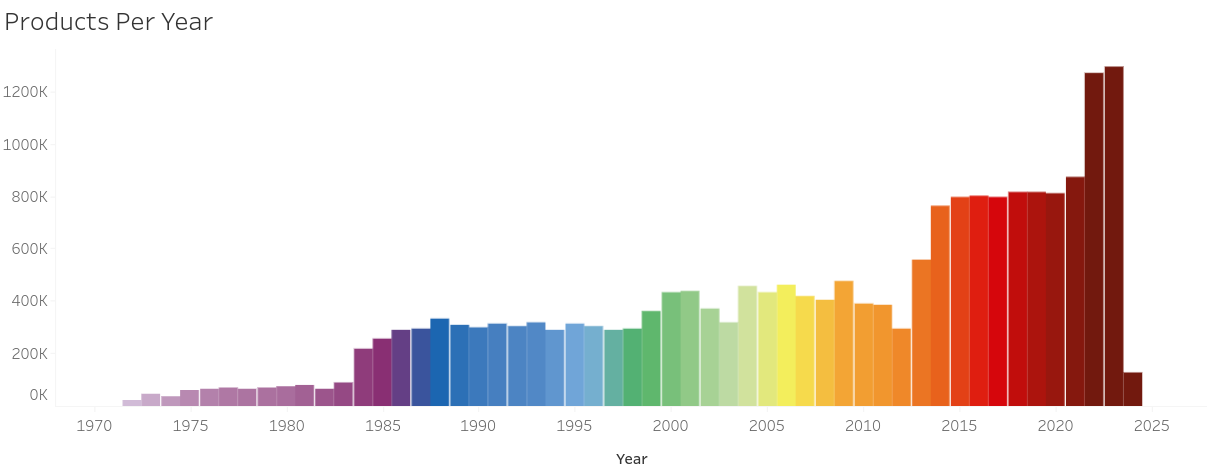
\includegraphics[width=\textwidth]{img/LandsatDataArchiveStatsProductsPerYear.png}
    \caption{Number of Landsat Products per year over time (as of Feb.2024) by the~\cite{landsatstats}\label{fig:landsatproductsovertime}}
  \end{figure}
  The rise in availability on the one hand makes it easier for researchers and companies to use the data, but requires increased computing and storage availability, to manage the increased data amount.
  This offers the possibility of creating scientific studies covering a wide range of cities over time, using the same sensor and tools. 
  \Cite{Sobrino2020} suggested a methodology to compare \glspl{UHI} using \gls{sentinel3}
  
  \subsection{Research Question}
    In this thesis the impact of change in land cover (urbanisation, urban development and other land use changes) and the impact of rising average temperature shall be investigated with regards to the urban heat island phenomena.

  \subsection{Methodology}
    % SUHI measurements using Thermal Infrared Satellite Data 
    
    % LULC impact using ML algorithm to create time lines of LULC of example cities

    % Measurment of UHI intesity over time 

    % Modelling of UHI into the future 

    % Application of different Indicies for measuring heat stress and other parameters for juding UHI intesity

    % Outlook and further research

  \subsection{Structure of the Thesis}
    In the introduction as well as \cref{sec:background} previous work and an overview of the current understanding of the urban heat island effect and research in this area is accessed. 
  %comparable definition
    \Cref{sec:definition} explains the used adaptation of the proposed methodology by~\cite{Sobrino2020} to create a definition of surface urban heat islands that is usable for comparing \glspl{UHI} in different cities.  
    \Cref{sec:LULC} explains how the measurements  and investigations of the impact of land use and land cover changes by build up where done.
    In \Cref{sec:UHITempImp} the impact of changing temperatures an increase of extreme weather phenomena on the intensity and seasonal variety of \glspl{UHI} was investigated. 
    After these the \cref{sec:conclusion} combines the findings of the previous chapters, shows what other investigations should be investigated further and where the research could be improved. 

   \section{Background}
\subsection{Urban Heat Islands}
The phenomenon of \acp{UHI} has been studied for the past 30 years. 
Due to increase in global temperature as well as increased occurrence of extreme weather and periods of heatwaves, this phenomenon will likely increase in intensity and will also occur in cities at higher latitudes~\cite{Sachindra2016}\cite[p.~904]{Wilby2008}.
\acp{UHI} are a spacial phenomenon that occurs on different scales and intensities, this makes observation using remote sensing data a good and widely used approach~\cite{Weng2003}.\\
\acp{UHI} are distinguished into surface and atmospheric \acp{UHI}.
Within this context we will only investigate surface \acp{UHI}. 
Surface \acp{UHI} are areas of higher surface temperatures within urban areas compared to rural areas due to the materials used and heat from mobility, electrical appliances, heating and cooling as well as less vegetation and higher sealed surfaces that reduce surface water availability\cite[pp. 7-12]{EPA2008}. 
The surface \acp{UHI} are longer term phenomenon that are most intense in summer. 
Atmospheric \acp{UHI} are more dependent on weather and local topology and are in part a side effect of the slower cooling of the city air due to the higher thermal capacity and wind obstruction.
This phenomenon is not investigated by this work, since the air temperature can not be directly observed by remote sensing data.
%Under certain conditions the increased temperature will form a hot air pocket, that will trap the head and reduce airflow from and to the area. \\
The main factors in forming urban heat islands is the thermal storage capacity of materials used in urban areas like concrete, asphalt and steel, that have a high heat capacity and heat up quickly during the day and emit the stored thermal energy as sensible heat with a delay (eg.~during the night)\cite{Ramamurthy2014}. 
High surface sealing and lack of vegetation reduce surface water availability and diminish evaporation and the cooling effect of latent heat causing more thermal energy to be available as sensible heat. %todo source (sailor?  or first source)
Another factor is the heat produced by human activity such as industrial processes and combustion engines.
As a consequence of higher temperatures, active cooling devices are more frequently used for buildings and vehicles. 
The emitted thermal energy of these heat pumps further increases the surrounding temperature, reinforcing the effect.
\\
There are multiple adverse effects and possible mitigation techniques for the mitigation and reduction of urban heat islands have been studied extensively since the 1970s\cite{Nichol1994}\cite{Stewart2011}. % list studies.  
Advective cooling can be observed when the temperature gradient generated airflow from the cooler surrounding areas towards the hot areas within the city, cooling it down\cite{HaegerEugensson1999}. \\
Urban areas with no close water body (generating sea breezes as well as latent heat transport) and with lower average wind speed are more likely to be affected by urban heat islands\cite{Ramamurthy2017}. 
Higher temperatures due to \acp{UHI} cause stress to animals and humans increasing health risk due to heat stroke and increased surface level ozone concentration\cite{Santamouris2020}.
\subsection{Land Surface Temperature}
Land surface temperature is the temperature at which an object emits infrared radiation according to plank's law\cite{Liang2020}. 
Using remote sensing methods this quantity can not be directly observed since the satellite is observing \ac{TOA} brightness temperature. 
This temperature can be transformed to a \ac{LST} using atmospheric correction and correction for the emissivity of the ground.
The conversion factor is data source dependent and can be found in \cref{sec:lstcalc}.


%\section*{Acknowledgements}

\section{Theoretical Background}
    \subsection{Indices}
Many different indices are used for analysis of images or parameters in remote sensing, atmospheric physics and meteorology.
The following sections introduce the indices that where used to analyse the \glspl{UHI} within this work. 
\subsubsection{NDVI}
\textit{The following section is a slightly reworked version of a section from the pre-thesis master project~\cite{andrae2023}}\\ 
%
\noindent
\begin{figure}[!htbp]
    \centering
    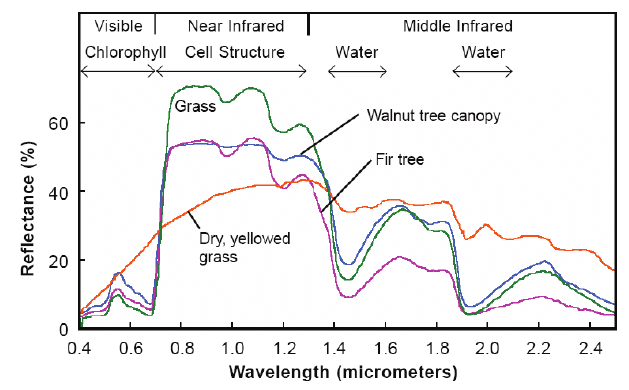
\includegraphics[width=0.5\textwidth]{img/Reflectance-spectra-of-different-types-of-green-vegetation-compared-to-a-spectral.png}
    \caption{Absorption spectrum of green vegetation \autocite[P. 5]{Smith2012}\label{fig:absorbtionVeg}}
\end{figure}
The \gls{NDVI} is an widely used index using the difference of the red and near infrared bands to determine the amount of green vegetation. 
\begin{equation}
    NDVI = \frac{Red-NIR}{Red+NIR}
    \label{equ:ndvi}
\end{equation}
For Landsat 8 and 9 data, channel 4 (red $640\ \text{nm} - 670\ \text{nm}$) and channel 5 (near infrared $850\ \text{nm} - 880\ \text{nm}$) where used.
As shown in \cref{fig:absorbtionVeg} healthy plants reflect near infrared and there is a sharp rise in reflectance between the two used channels at around $700\ \text{nm}$. 
%
This index is used for emissivity estimation for Land Surface Temperature calculation see \cref{equ:toa}, correlation with heat islands (since there is a negative correlation between those two values, due to the latent heat of evaporation reducing surface temperature at higher vegetation areas).
\begin{figure}[!htbp]
    \centering
    \begin{subfigure}{0.45\textwidth}
    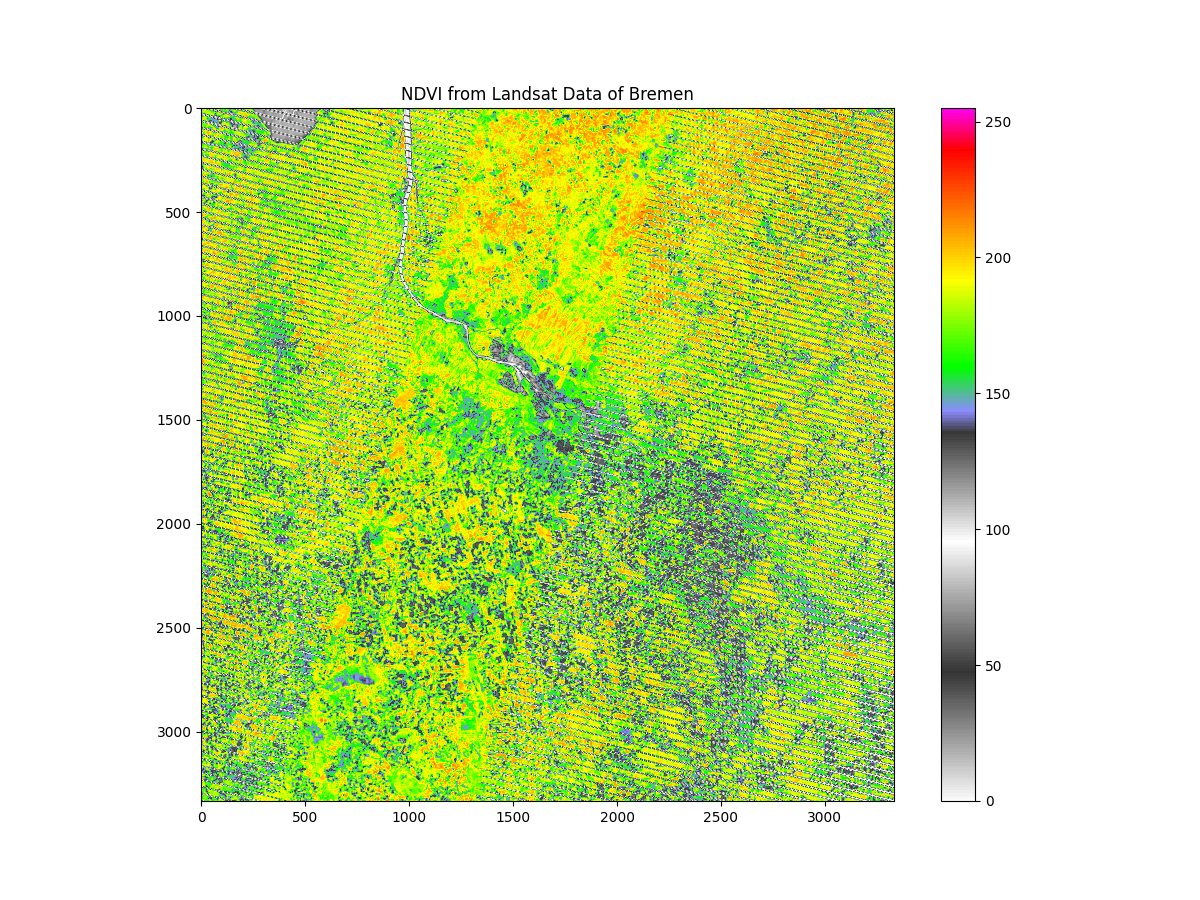
\includegraphics[width=\textwidth]{img/NDVI_LE07_L1TP_196023_20190723_20200825_02_T1__Bremen.png}
    \subcaption{NDVI of Bremen (Bands 5 and 6) using Landsat 7 data on 2019--07--23}
    \end{subfigure}
    \begin{subfigure}{0.45\textwidth}
    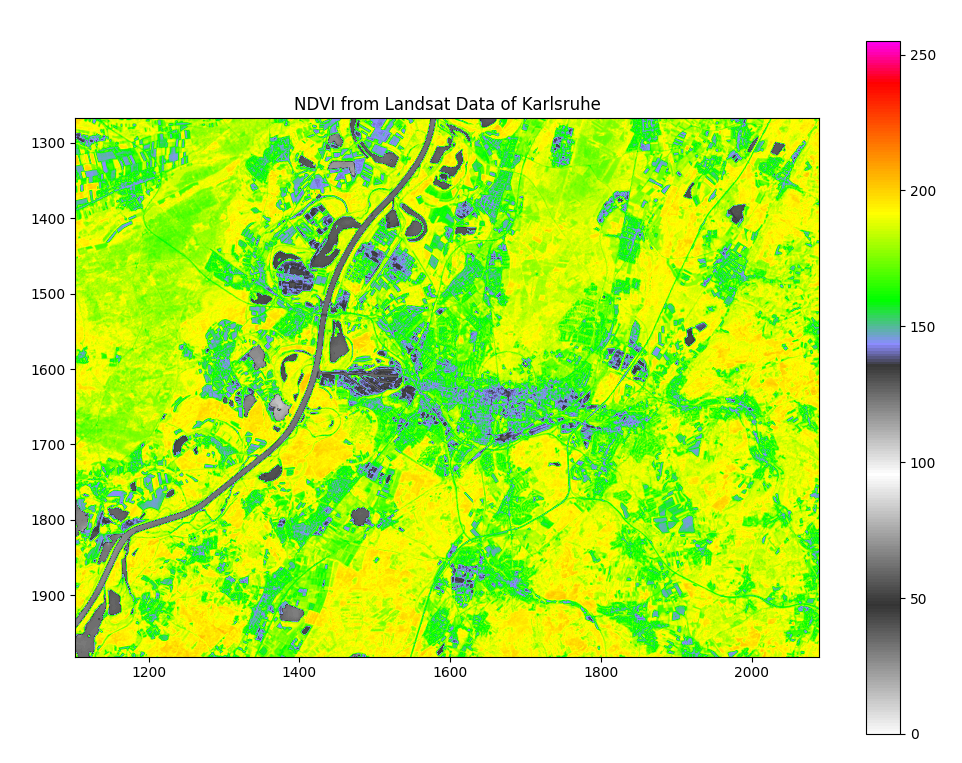
\includegraphics[width=\textwidth]{img/KarlsruheNDVI_Landsat8.png} 
    \subcaption{NDVI of Karlruhe (Bands 4 and 5) using Landsat 8 data on 2023--06--07}
    \end{subfigure}
    \caption{NDVI Images from the different satellites\label{fig:ndvi}}
\end{figure}
%\subsubsection{NDVI Colormap}\label{sec:colormap}
%When using a classical heat map with a color gradient from colder to warmer colors or a diverging color map (see \cref{fig:ndviPhoenixAzBad}), details of the image get lost and it is hard to distinguish plant heath, build up and vegetated areas and the difference between small \gls{NDVI} changes.
%To aid an intuitive understanding a specially created colormap can be used. 
%The color map was adapted for use in python from work of \texttt{public lab}\cite{ndviCmap} where it was developed in an attempt to create color-blind friendly \gls{NDVI} color maps.
%Values below 0.2 are areas with no vegetation.
%The color map used in \cref{fig:ndviPhoenixAz} uses a gradient of gray with a ``black-white-black
%white'' transition to allow higher dynamic range for non vegetation areas.
%For areas with an \gls{NDVI} $<$ 0.2 blue is used. Green values are low or unhealthy green vegetation or mixed use pixels. 
%Orange and red values correspond to thicker vegetation e.g.~forests, parks or green fields. 
%%
%Comparing \cref{fig:ndviPhoenixAz}  and \cref{fig:ndviPhoenixAzBad} where most of the desert surrounding the city has no green vegetation and the parts covered in vegetation can be clearly distinguished from the arid desert regions.
%Still the surface roughness can be seen quite well due to the gray scale gradient in the $<$ 0.2 \gls{NDVI} range.  
%%
%\begin{figure}[htbp]
% \centering
%    \begin{subfigure}{0.46\textwidth}
%    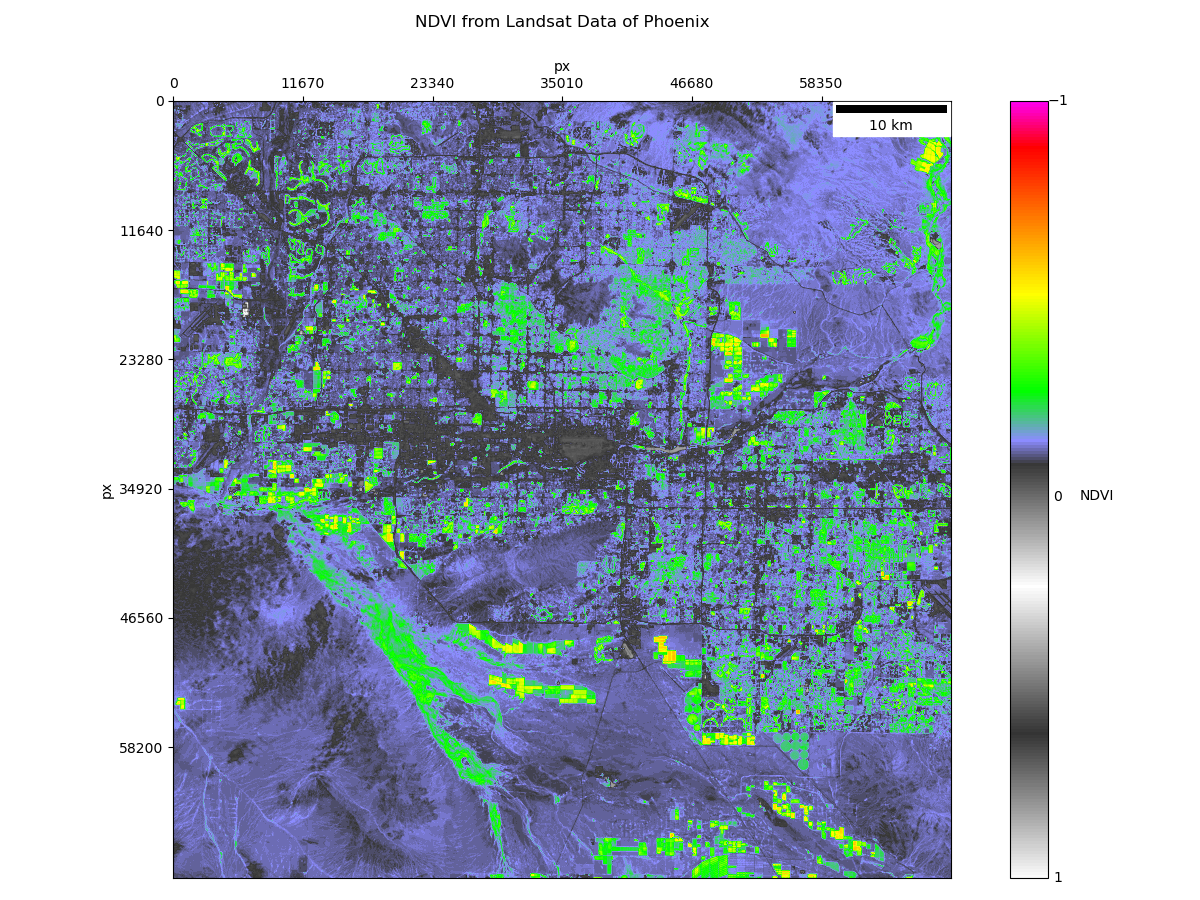
\includegraphics[width=\textwidth]{img/NDVI from Landsat Data of Phoenix.png} 
%    \subcaption{NDVI Image of Phoenix with the  VGYRM color map\label{fig:ndviPhoenixAz}}
%    \end{subfigure}
%    \begin{subfigure}{0.46\textwidth}
%    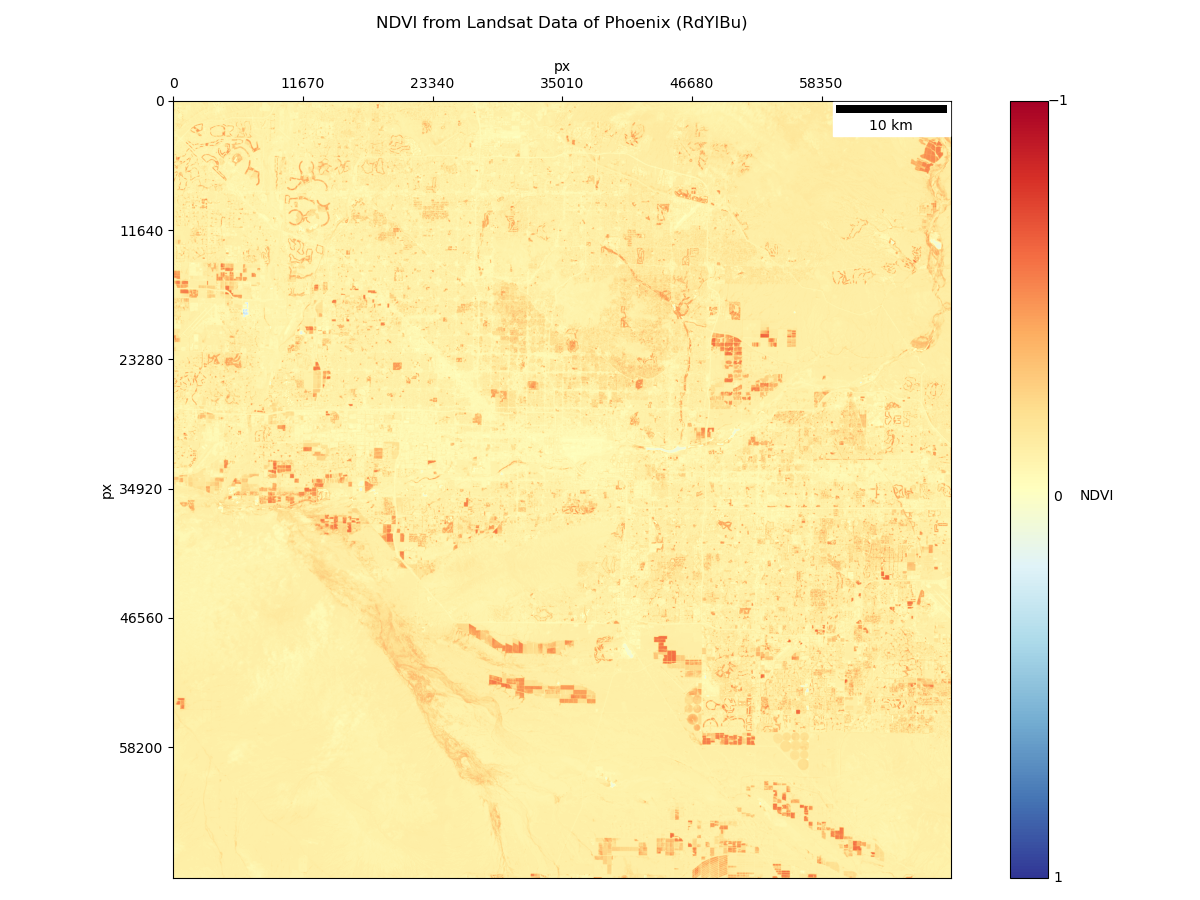
\includegraphics[width=\textwidth]{img/NDVI from Landsat Data of Phoenix (RdYlBu).png} 
%    \subcaption{NDVI Image of Phoenix with a RdYlBu gradient color map\label{fig:ndviPhoenixAzBad}}
%    \end{subfigure}
%    \caption{Different color maps used show the better ability to differentiate between green vegetation and desert and buildings within Phoenix\label{fig:ndvicomp}}
%\end{figure}

    \newpage
    \subsubsection{Heat Index}
    The \gls{HI}is a temperature index that takes sultriness into account and rates the impact of temperature and air humidity of the human body. 
    The output of this temperature scale (given in °C) is the apparent temperature, depending on relative air humidity. 
    The defined range is between 20 °C and 50°C dry bulb temperature and up to 90\% relative humidity~\cite[p. 862]{Steadman1979}. 
    The proposed heat index is based on a model human and takes wind chill and clothing into account, to produce a apparent temperature of human. 
    The heat index can be used as a good reference for non-extreme conditions. 
    Its biggest downside is the missing account for direct insolation on body temperature and comfort.
    The Heat Index later is used to compare different \glspl{UHI} with each other.


    \subsubsection{Wet Bulb Globe Temperature}
    To account the impact of insolation on the human body and how it reacts to heat stress differently in different environmental conditions, the Wet Bulb Globe Temperature was developed. 
    Working under heat stress poses a serious health issue, for this the \gls{WBGT} was defined as EN ISO 7243:2017, calculating the thermal load on the human body\cite{Iso7243_2017}
    Heat exchange between the human body and the environment is dominated by evaporation of secreted sweat.
    The efficiency of this process is determined by the vapor pressure, that is influenced by temperature difference and the humidity difference. %TODO ref paper with caves
    The Heat Index is a simple way of calculating this efficiency that does not take radiant heat into account, the WBGT does incorporated this effect as well as clothing in this process. 


    \subsubsection{Urban Air Quality}
    Large urbanized areas are susceptible to air pollution due to increased combustion and industrial activity. % TODO Numerous studies \cite{Kanakidou2011}
    One major pollutant with a significant health impact is tropospheric ozone that is produced in larger quantities within higher temperature environments (see~\cite{Ebi2008}). 
    Ozone is mainly produced when (anthropogenic) NO\textsubscript{x} emissions and other \glspl{VOC} react with volatile organic compounds. %todo source
    The creation of ozone is dependent on temperature, increasing between 2.2 and 3.2 ppbv/°C depending on NO\textsubscript{x}

    %\subsection{Models and Theories}
    \section{Image Processing}\label{sec:imgProcessing}
    Using remote sensing data for scientific purposes requires a (a) systematic, (b) reproducable, (c) verifiable way of detecting patterns and information within the data. \\ 
    The field of image processing and machine learning has developed a wide range of tools that are used in many different fields over the past decades. % TODO might want to add examples here ?

    \subsection{Machine Learning}\label{sec:ml}
    The term machine learning describes a set of algorithms that use a set of training data, detect statistical correlations using different weights to approximate this data. %TODO external source 
    These approximations can be stored and be used to detect the same features within new but similar data.
    
    In the next sections the image processing steps are described from a technical perspective and the underlying mathematical frameworks are discussed.
    \subsection{Data Processing Pipeline}
    An image or data processing pipeline is a chained list of processing steps, that allows to feed different data through the same algorithm. 
    Many different data processing and machine learning \glspl{lib} use these to allow flexibility and modularity of the steps in data processing (e.g.\ the used~\cite{scikit},~\cite{keras} or~\cite{gluon}). 
    The data processing was used using scikit-learn pipeline for data analysis as well as multiple other \glspl{lib}. 
    In \cref{fig:pipeline} the overview of the different steps within the data processing can be seen.

    \begin{figure}[!htbp]
       \centering
     \begin{subfigure}[b]{\textwidth}
         \centering
         \begin{tikzpicture}[node distance=2cm, auto, scale=.5, on grid]
  \node (start) [startstop, text width=0.7\textwidth] {Start};
  \node (input) [io, below of=start, text width=0.6\textwidth]{Landsat 8\ \& 9 Image};
  \node (cut) [process, below of=input, text width=0.9\textwidth]{Cut to AOI};
  \node (features) [process, below of=cut, text width=0.9\textwidth]{Gabor Feature Extraction};
  \node (kmeans) [process, below of=features, text width=0.9\textwidth]{KMeans clustering};
  \node (stat1) [process, below of=kmeans, text width=0.9\textwidth]{Statistical analysis of different classes};
  \node (stat2) [process, below of=stat1, text width=0.9\textwidth]{manual class name assignment};
  \node (verif) [process, below of=stat2, text width=0.9\textwidth]{verification of classification};
  \node (diff) [process, below of=verif, text width=0.9\textwidth]{diff analysis of LU/LC classes};
  \node (stop) [startstop, below of=diff,text width=0.7\textwidth] {Stop};

  \draw[arrow] (start) -- (input);
  \draw[arrow] (input) -- (cut);
  \draw[arrow] (cut) -- (features);
  \draw[arrow] (features) -- (kmeans);
  \draw[arrow] (kmeans) -- (stat1);%(randomforest);
  %\draw[arrow] (randomforest) -- (stat1);
  \draw[arrow] (stat1) -- (stat2);
  \draw[arrow] (stat2) -- (verif);
  \draw[arrow] (verif) -- (diff);
  \draw[arrow] (diff) -- (stop);
\end{tikzpicture}

         %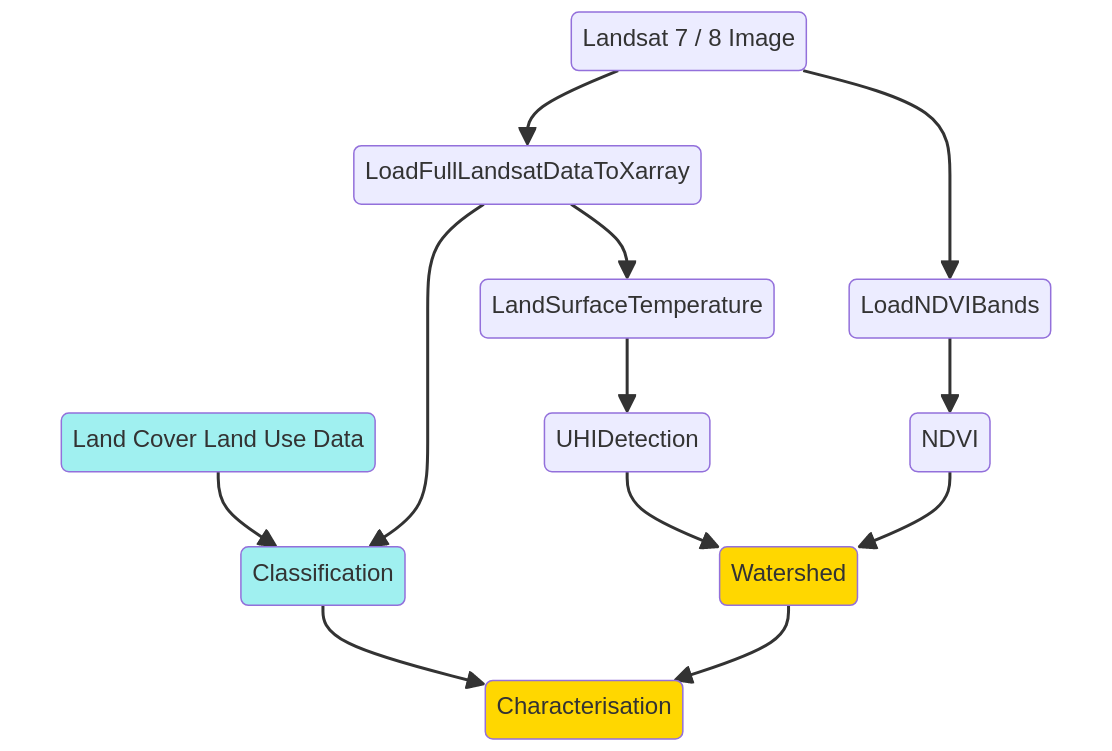
\includegraphics[width=\textwidth]{img/DiagPipeline.png}
         \caption{Processing pipeline for developing the model}\label{fig:pipelineTraining}
     \end{subfigure}

     \begin{subfigure}[b]{\textwidth}
         \centering
         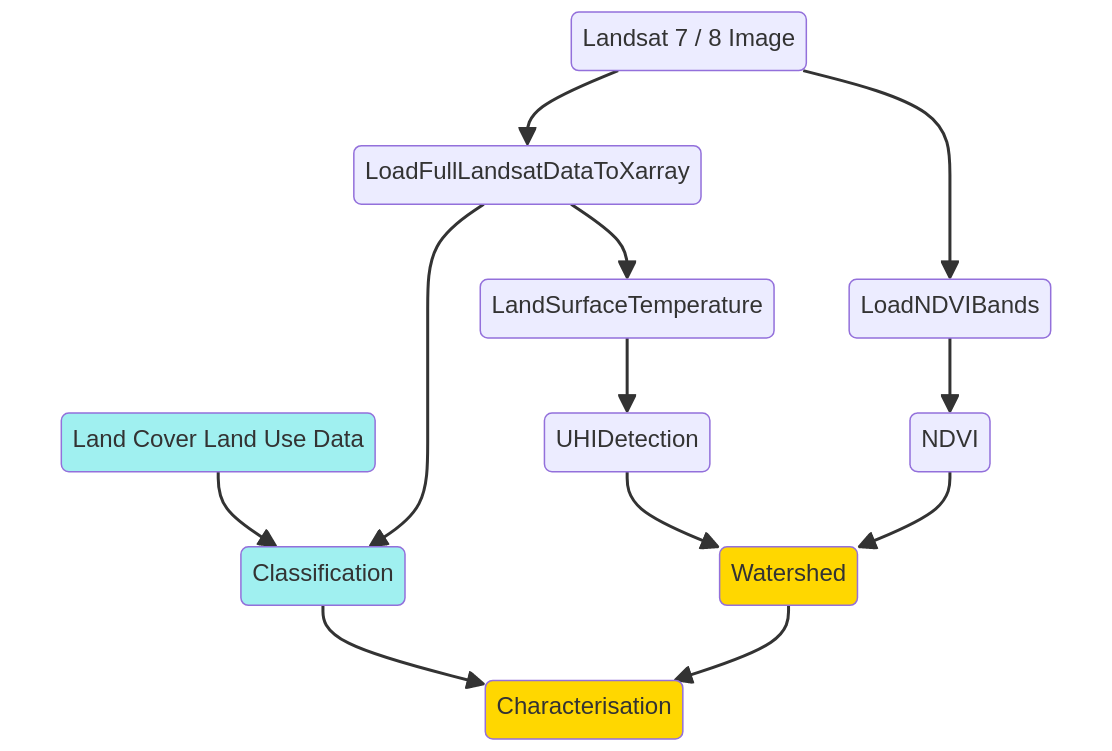
\includegraphics[width=\textwidth]{img/DiagPipeline.png}
         \caption{Data Processing pipeline with the trained Model}\label{fig:pipelineTrained}
     \end{subfigure}
     \caption{The image processing overview\label{fig:pipeline}}
     \end{figure}

    \subsection{Gabor Feature Detection}\label{sec:gabor}
    The Gabor filter is an linear filter, that uses a convolution of an image with a wavelet created by rotating a sine modulated gaussian, this kernel type is also called the \textit{gabor wavelet}. 
    In image processing this algorithm is used as an feature extraction algorithm to extract and analyse texture and structures with different sizes within the image~(\cite{Cerdan1993}). 
    By rotating the kernel and changing the frequency, different textures are extracted from the image.
%
    Mathematically the Gabor-filter is defined by
    \begin{equation}
      g(x,y; \lambda, \theta, \phi, \sigma, \gamma) = \exp \left(- \frac{x'^2 + \gamma^2\cdot y'^2}{2\sigma^2}\right) \cdot \exp \left[i \left(2\pi\frac{x}{\lambda} + \phi \right)\right] 
    \end{equation}
    With $ x' = x \cos(\phi) + y \sin(\phi)~\text{and}~y' = -x \sin(\phi) + y \cos(\phi)$.
%
    The x and y parameter determine the kernel size, this parameter should be chosen based on the image size and expected structure length.\\
    $\gamma$ is the aspect ratio of the kernel, with $\gamma = 1$ the kernel is round, for smaller $\gamma$ the kernel becomes a more eccentric ellipse.\\
    $\phi$ is the angle of rotation of the sine component of the kernel. \\
    $\theta$ is the angle of rotation of the kernel, detecting differently oriented features.\\
    $\lambda$ is the wavelength of the sine wave. \\
    $\sigma$ is the standard deviation of the Gaussian distribution\\ 

    
    %TODO add more accurate description of parameters
%
    To detect different structures of different scales within the image, a filter bank can be created by combining multiple filters and varying $\phi$, $\sigma$ and $\theta$.\\
%
    After the convolution of the image with the filter bank, the resulting set of detected features can be used as an input into different algorithms.
    \Cref{fig:gaborExample} shows different kernel sizes and rotations on an satellite image of Bremen. 
    It can be seen that the different structures such as fields (seen in \cref{fig:feat02} and \cref{fig:feat05}) or larger structures and water bodies (seen in \cref{fig:feat01} and \cref{fig:feat03}).
    The output of the filter is an tensor that contains a binary image sized matrix per filter. Each layer provides meta information for each pixel, if it is part of a larger scale texture or pattern. 
    This meta information is used in surface classification (\cref{sec:classification}).

    \begin{figure}[!htbp]
       \centering
     \begin{subfigure}[b]{0.3\textwidth}
         \centering
         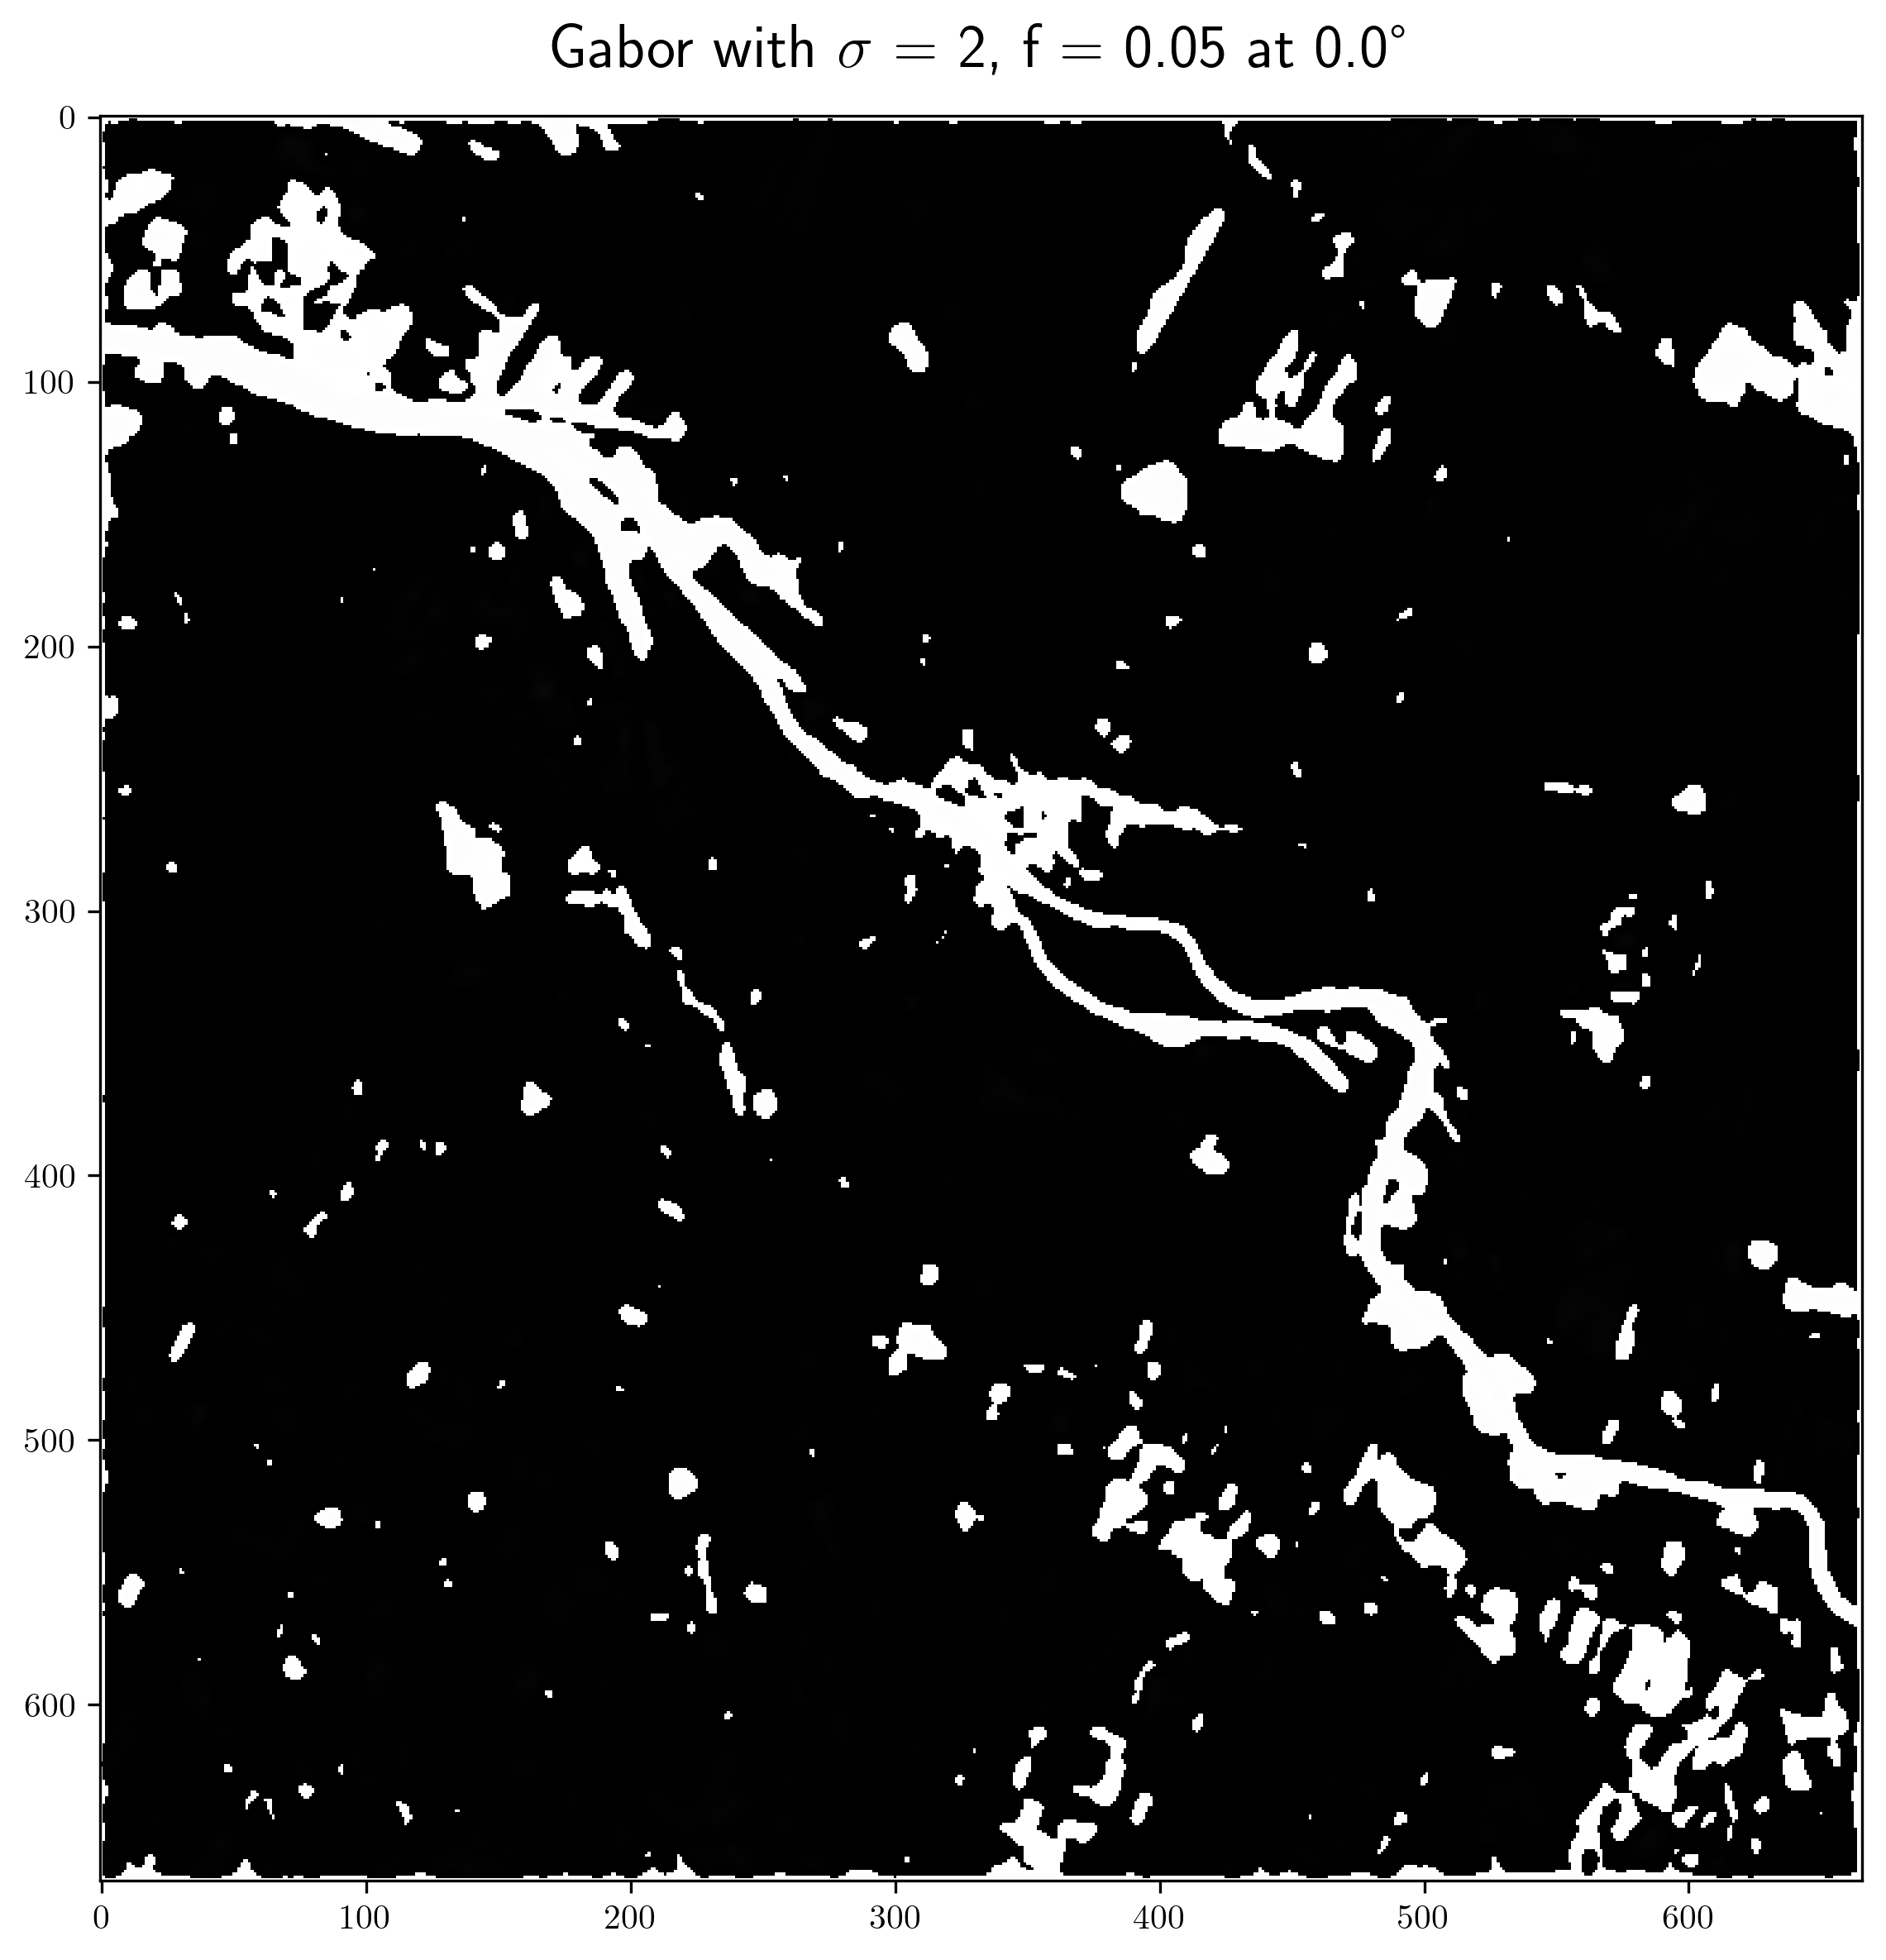
\includegraphics[width=\textwidth]{img/Features_2_005_0.png}
         \caption{Kernel with $\sigma$ = 2, f = 0.05 and 0 ° rotation}\label{fig:feat01}
     \end{subfigure}
     \hfill
     \begin{subfigure}[b]{0.3\textwidth}
         \centering
         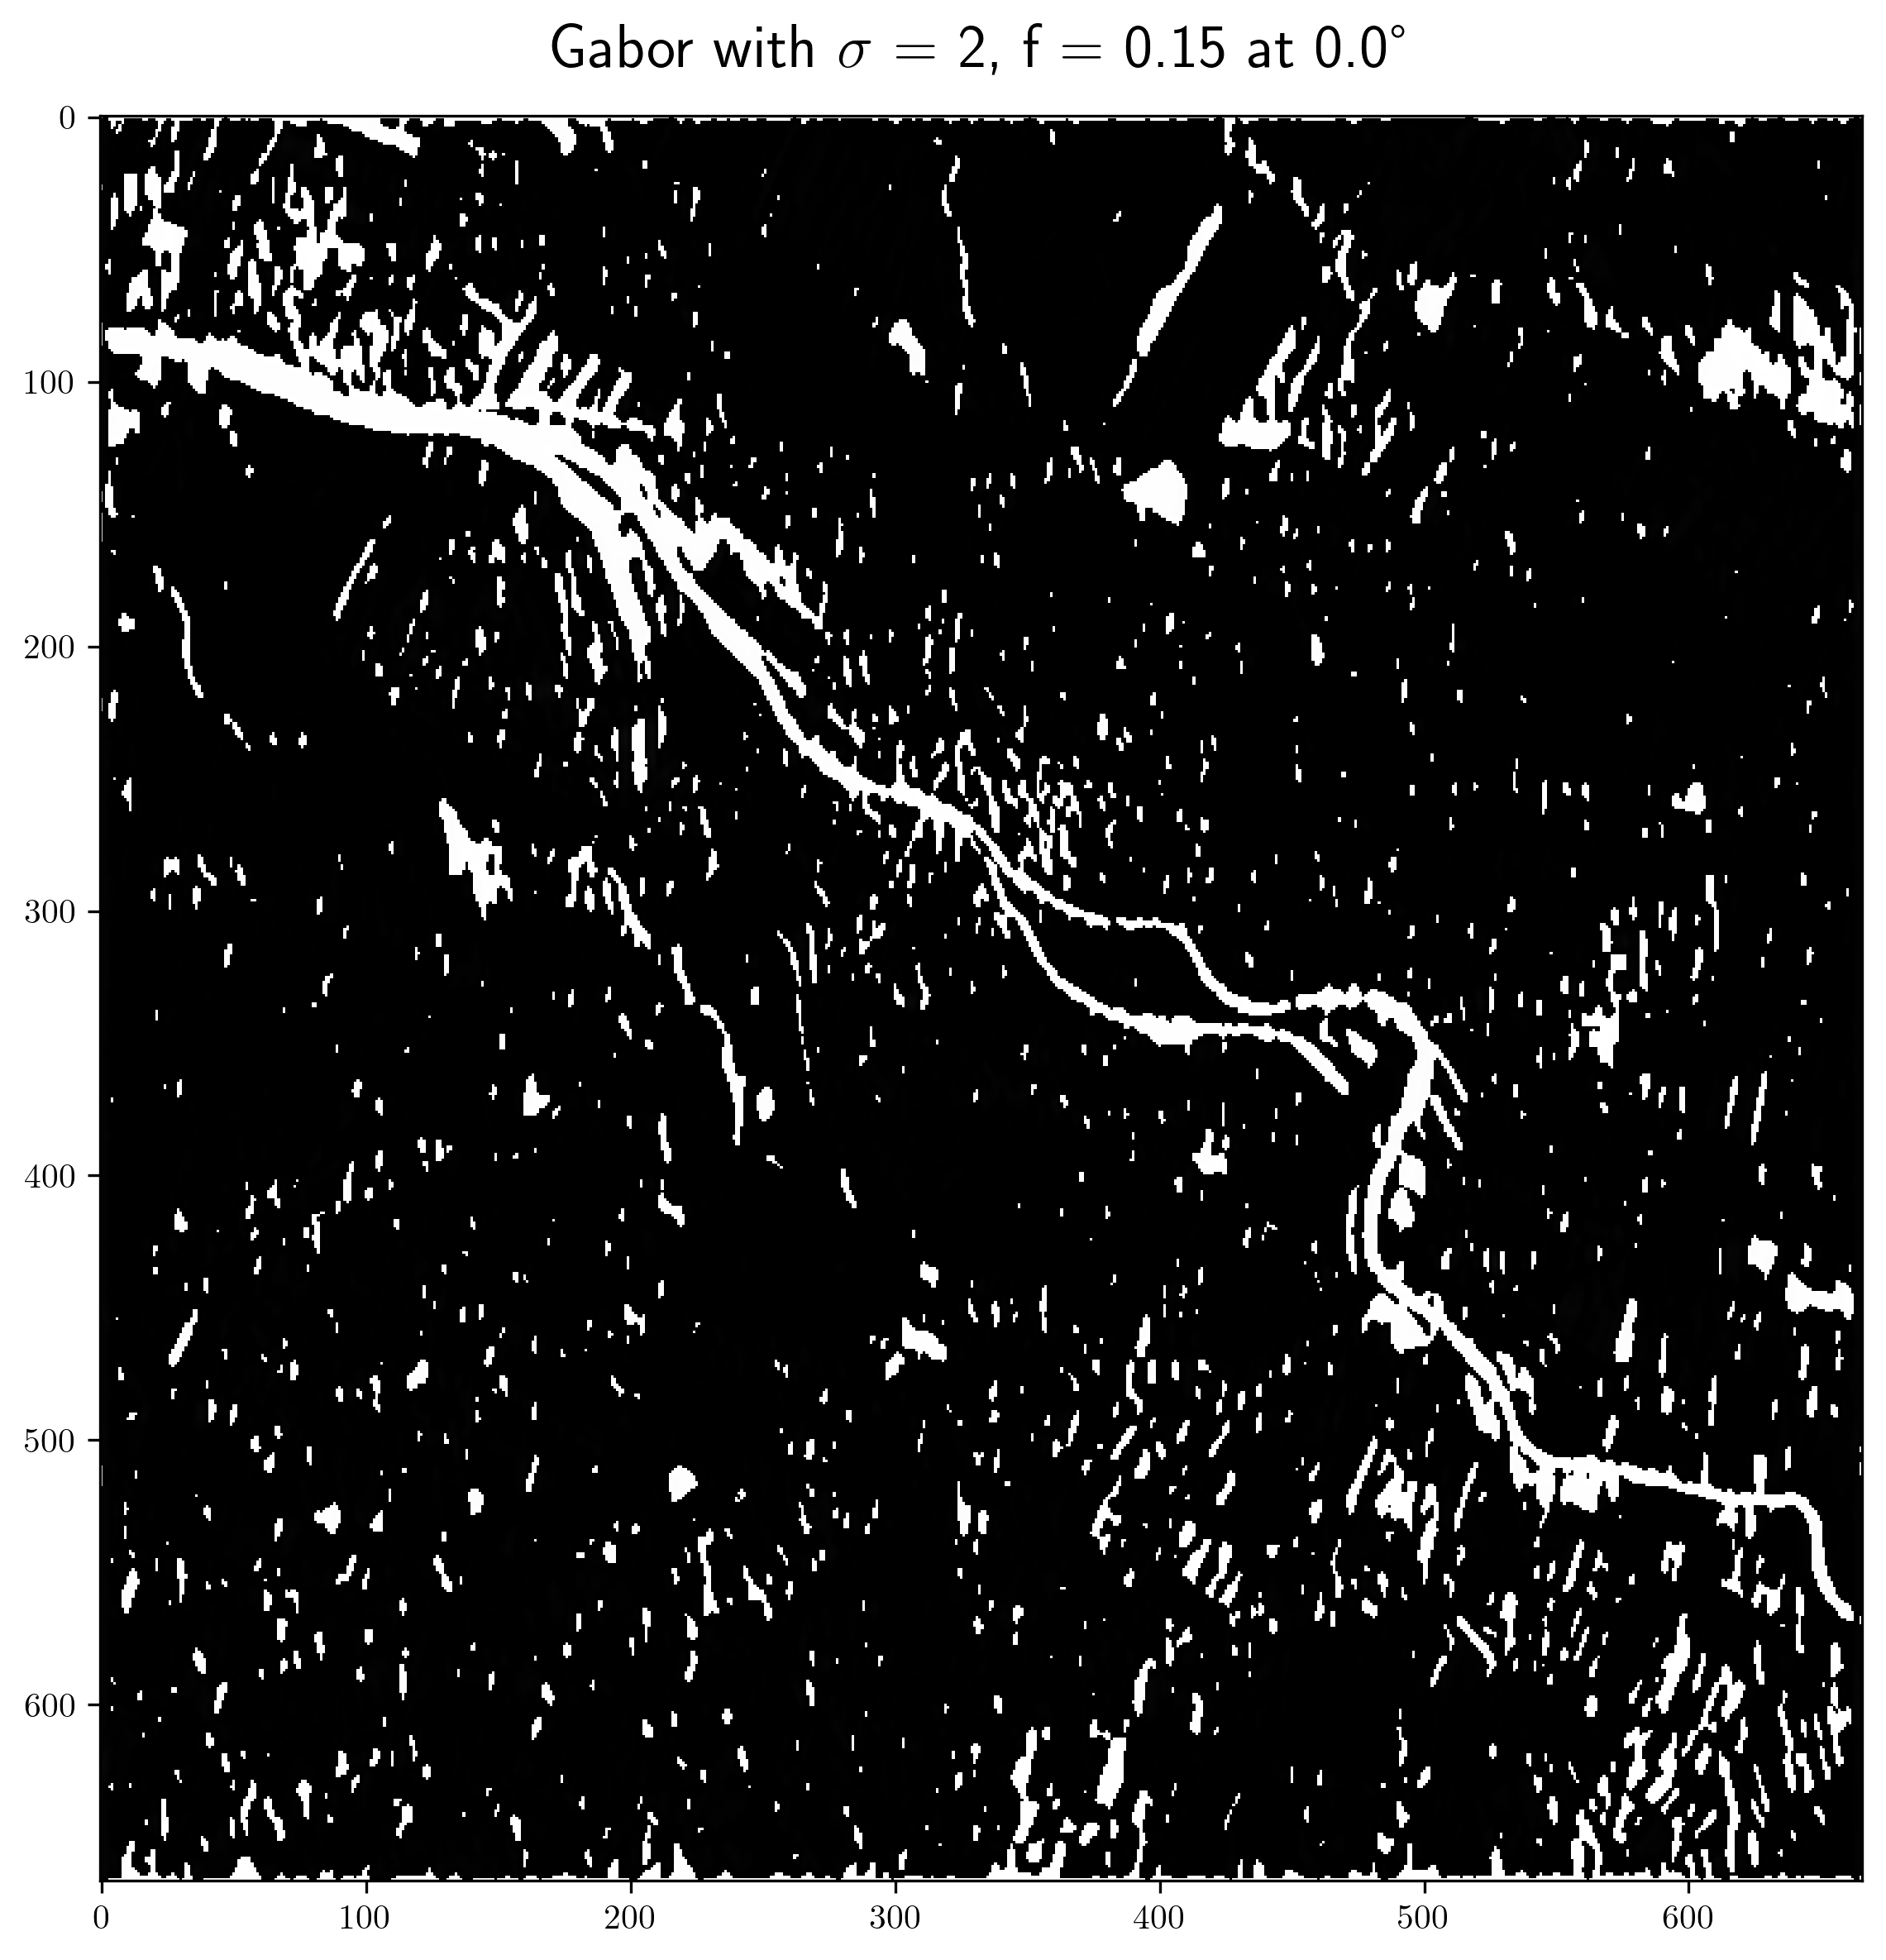
\includegraphics[width=\textwidth]{img/Features_2_015_0.png}
         \caption{Kernel with $\sigma$ = 2, f = 0.15 and 0 ° rotation}\label{fig:feat02}
     \end{subfigure}
     \hfill
     \begin{subfigure}[b]{0.3\textwidth}
         \centering
         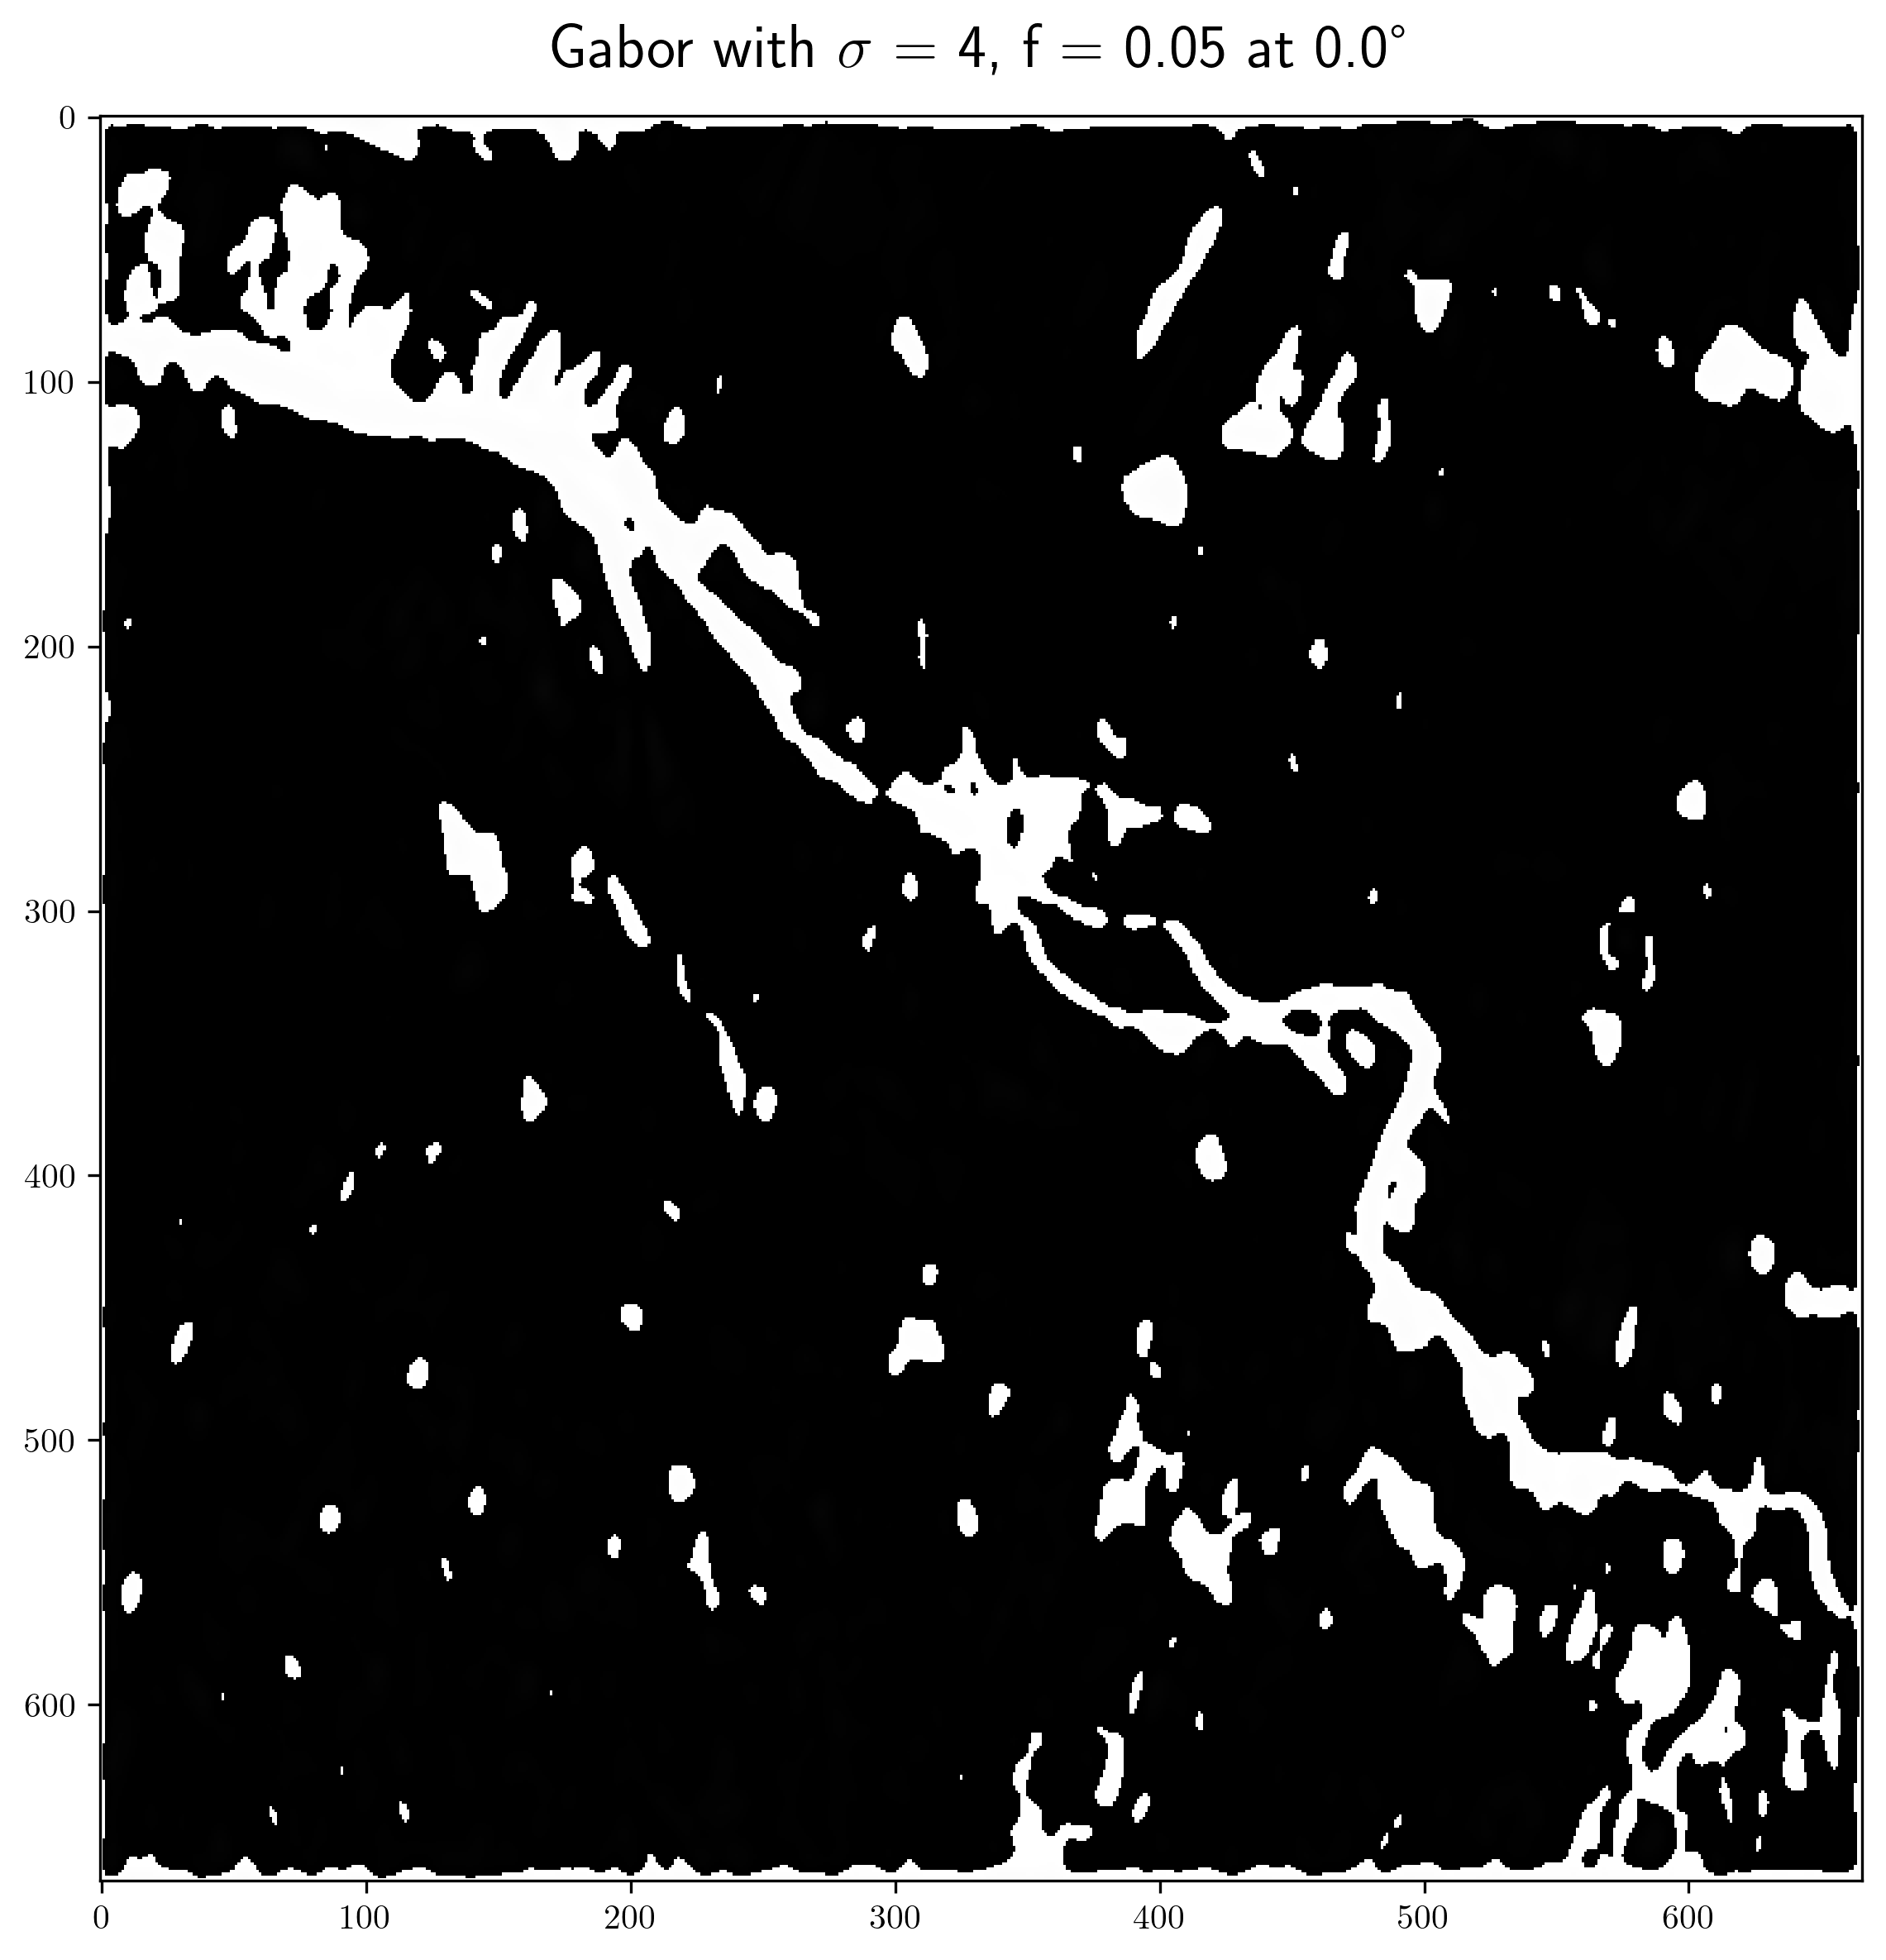
\includegraphics[width=\textwidth]{img/Features_4_005_0.png}
         \caption{Kernel with $\sigma$ = 4, f = 0.05 and 0 ° rotation}\label{fig:feat03}
     \end{subfigure}

     \begin{subfigure}[b]{0.3\textwidth}
         \centering
         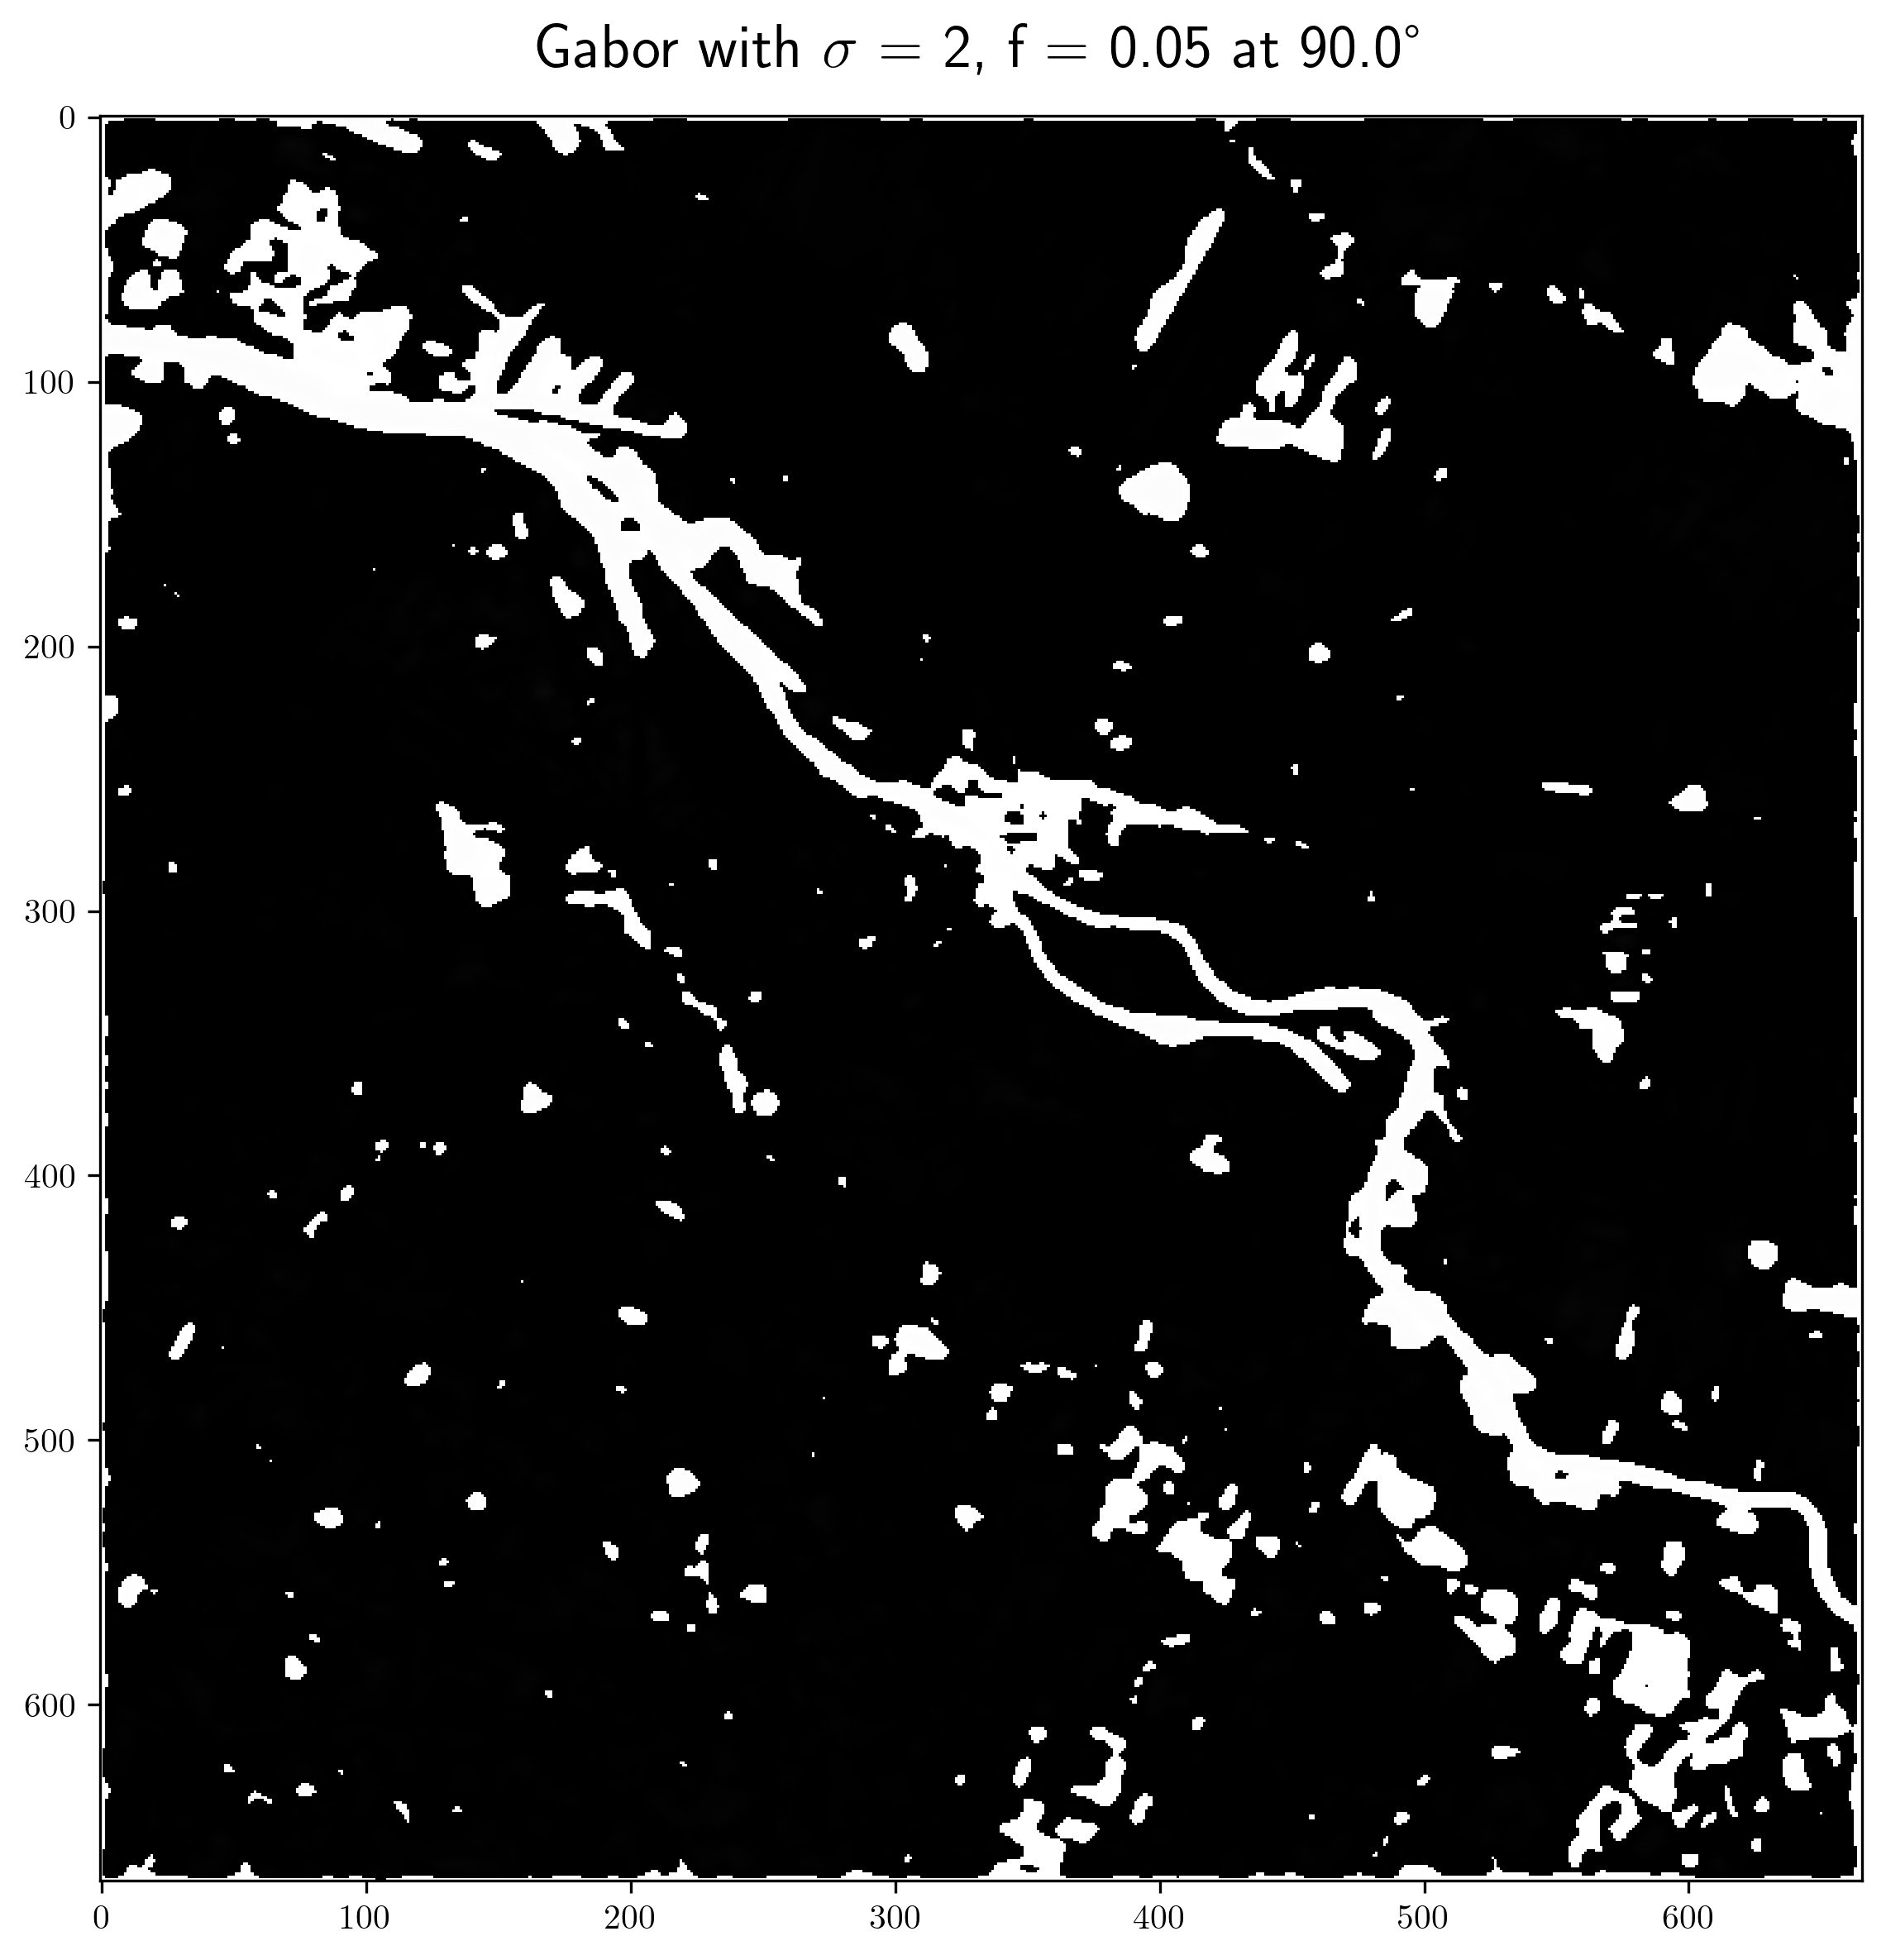
\includegraphics[width=\textwidth]{img/Features_2_005_90.png}
         \caption{Kernel with $\sigma$ = 2, f = 0.05 and 90 ° rotation}\label{fig:feat04}
     \end{subfigure}
     \hfill
     \begin{subfigure}[b]{0.3\textwidth}
         \centering
         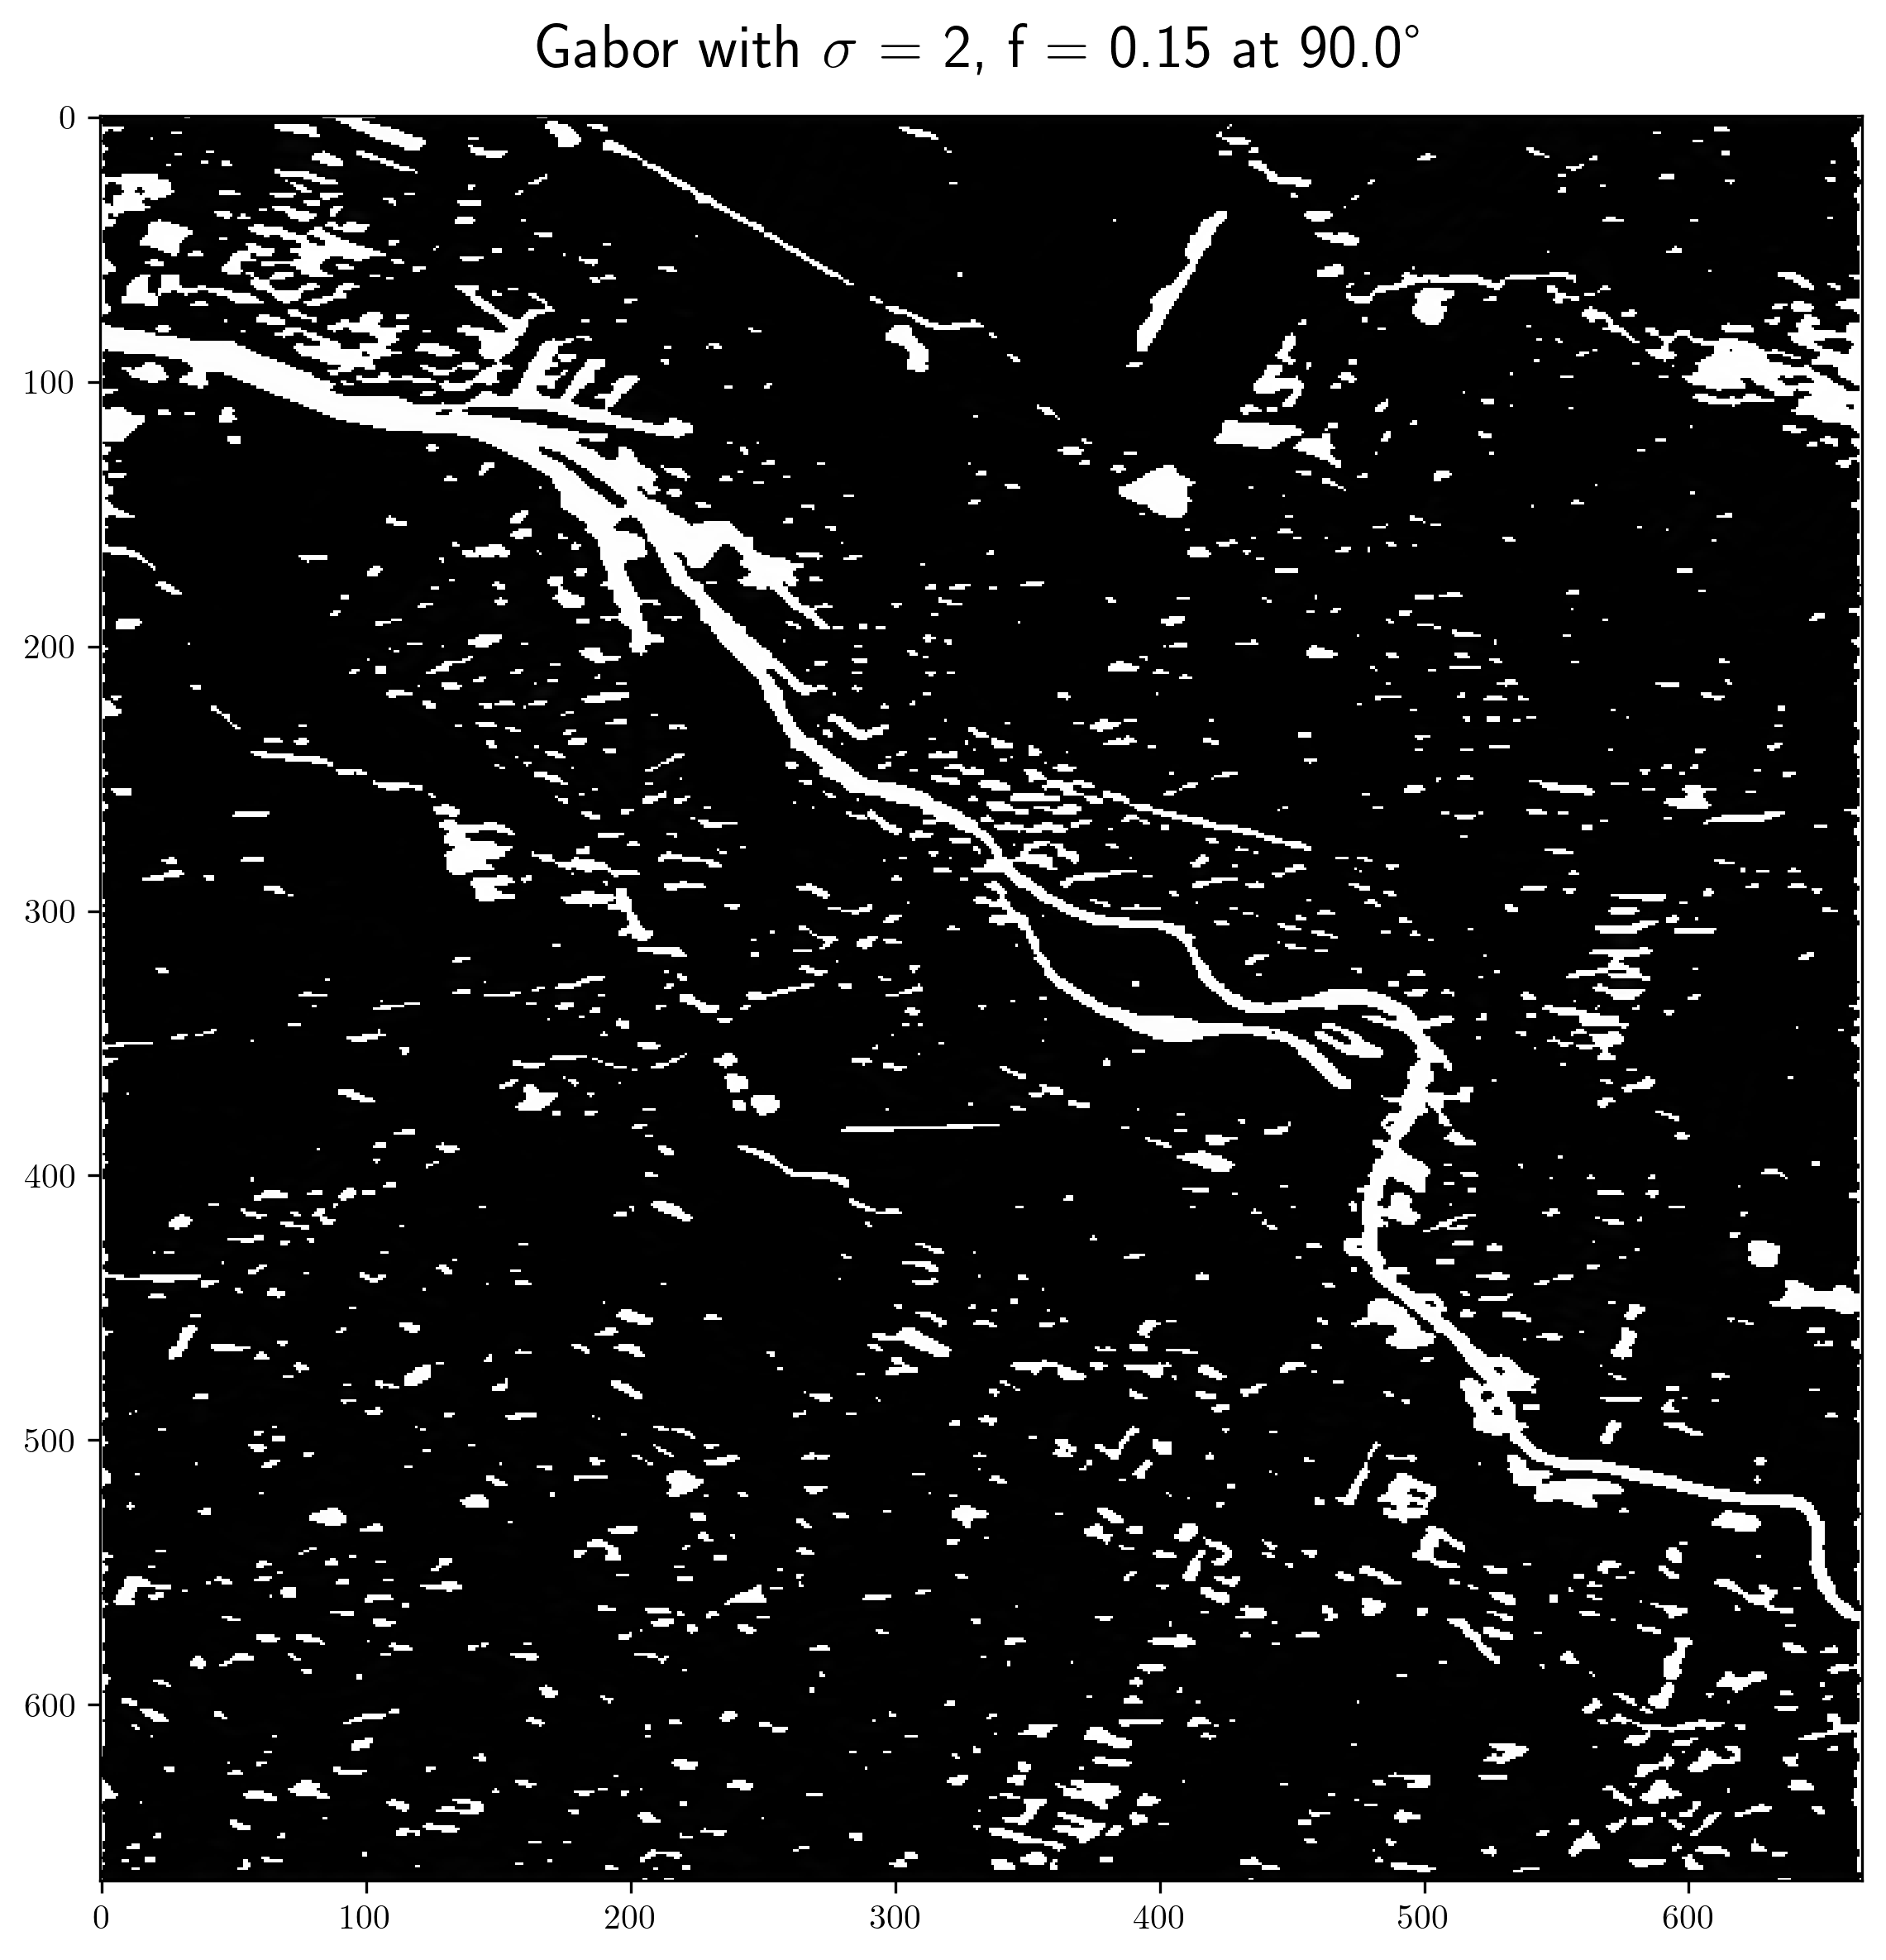
\includegraphics[width=\textwidth]{img/Features_2_015_90.png}
         \caption{Kernel with $\sigma$ = 2, f = 0.15 and 90 ° rotation}\label{fig:feat05}
     \end{subfigure}
     \hfill
     \begin{subfigure}[b]{0.3\textwidth}
         \centering
         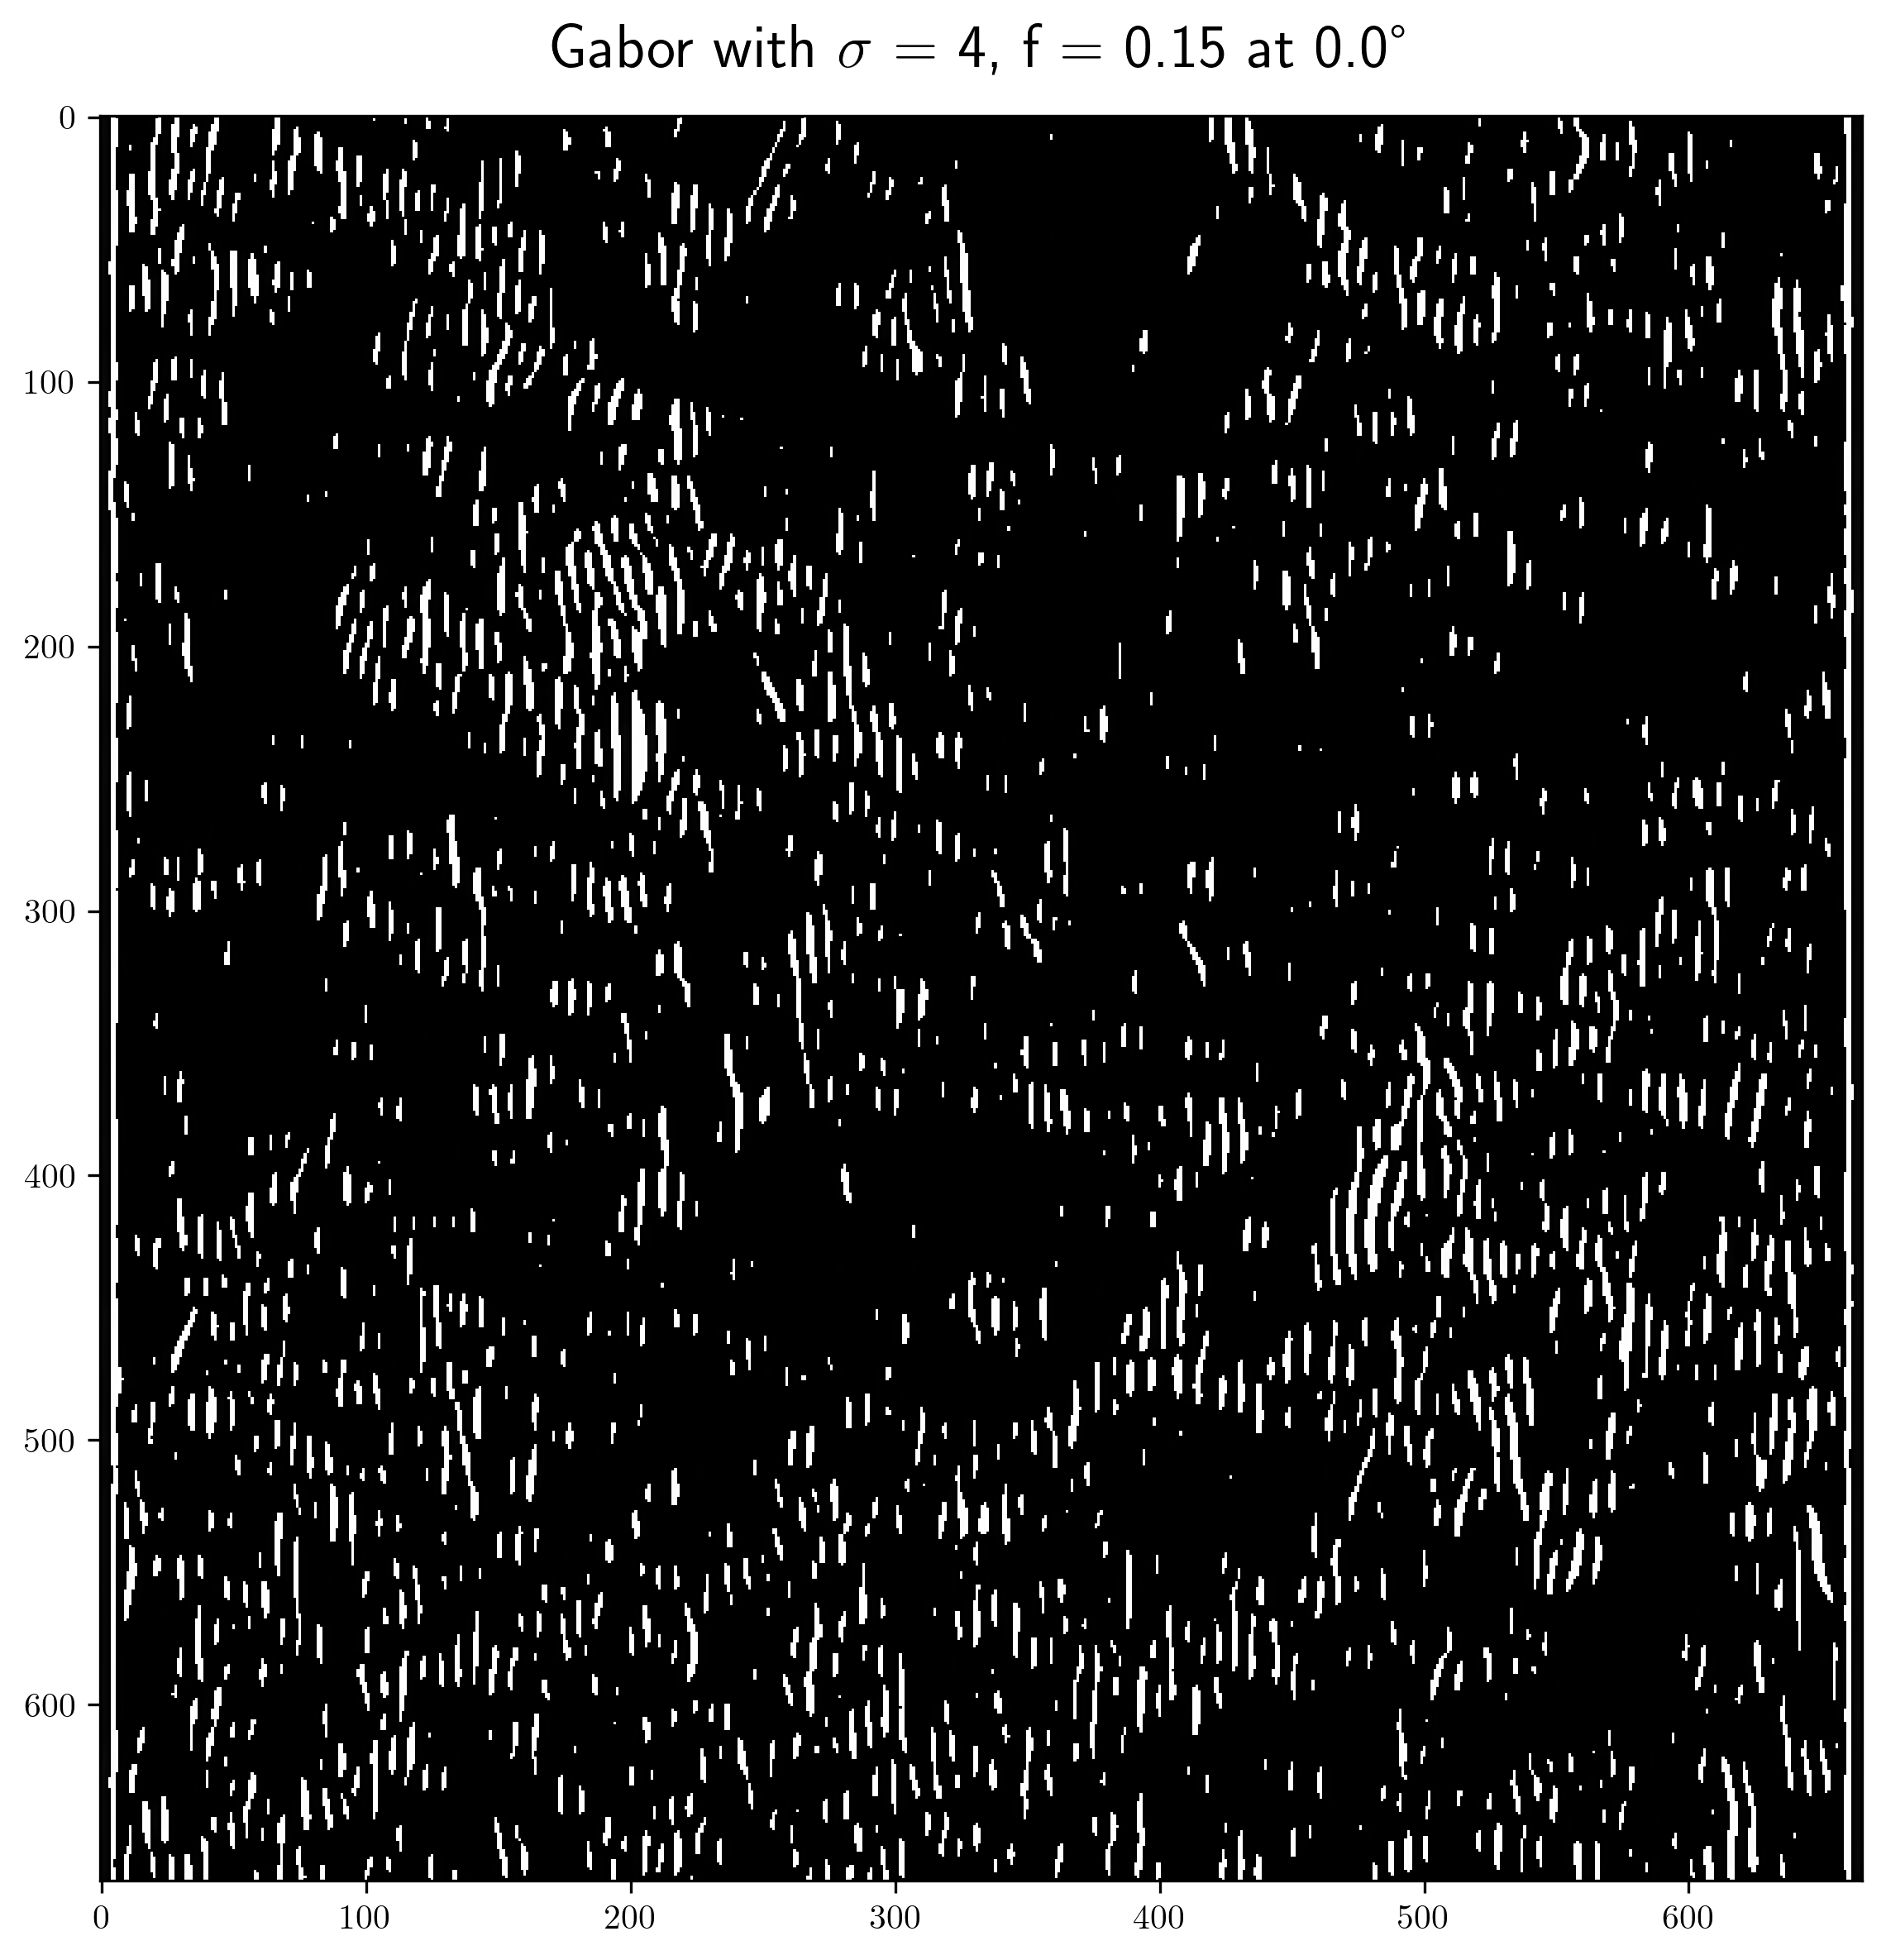
\includegraphics[width=\textwidth]{img/Features_4_015_0.png}
         \caption{Kernel with $\sigma$ = 4, f = 0.15 and 0 ° rotation}\label{fig:feat06}
     \end{subfigure}
        \caption{Result of convolving differently oriented gabor wavelets with an Landsat-8 image of Bremen}\label{fig:gaborExample}
    \end{figure}




    \section{Comparable Definition of Urban Heat Islands}\label{sec:definition}
    \subsection{Introduction}
    The definitions of \glspl{UHI} in the literature are varying slightly and do not take into account that, using remote sensing techniques most definitions do not allow easy comparison between different areas or times.
    %TODO add sources, maybe add examples? 
    The definition of the U.S.~EPA\cite{EPA2008} and the German Weather Service (DWD) both say it is an feature defined by increased temperature between the urbanized areas compared to the sourrounding. % TODO cite  
    Different studies analyzing \glspl{UHI} use difference referenece tempereatures.
    The first goal of this work is defining a systematic reproducable aproach to measure urban heat island intensity based on land usage.

    \subsection{Approach}
    To make the approach comparable previous work was done tackeling the problem using a comparable definition for comparing \gls{SUHI} around the world using Sentinel images\cite{Sobrino2020}.
    The land cover classes indicating urban areas is identified and the urban area polygon is extended by buffer zones. 
    \begin{figure}
      \includesvg[width=\textwidth]{img/UrbanAreaBremen}
      \caption{Urban Area of Bremen, with buffer zones for Adjacent and Peri Urban Area}
    \end{figure}
    In~\cite{Sobrino2020} urban adjacent, future urban adjacent and peri-urban areas are defined.
    The used approach was adapted by removing the urban growth projection (the paper investigated \glspl{SUHI} in 2050).
    For \gls{LULC} Landsat 8/9 data was used combined with different \gls{ML} techniques for surface classification (see \cref{sec:classification}). % TODO 

    
    \subsubsection{Used Satellites}
    Using remote sensing data to detect and analyse \gls{SUHI} requires devices that detect thermal infrared radiation. 
    Satellites that are equipt with thermal infrared sensors that are able to detect upwelling emmission from the surface temperature within the $ 8 < \lambda < 12 \mu m $ range. 
    Commonly used instruments used for measuring \glspl{UHI} are Landsat, MODIS, ASTER and Sentinel-3. 
    
    \subsection{Analysis}
    \subsubsection{Land Surface Temperature Calculation}\label{sec:lstcalc}
    The \gls{LST} can not be measured directly by a satellite but must be calculated from the upwelling thermal infrared radiation and corrected for the atmospheric perturbation. For Landsat 7 and Landsat 8 data is provided in different processing levels.
    The Level 1 data provides \gls{TOA} brightness and is corrected for stray light (Landsat 8 specific, see~\cite[p.~67]{Zanter2019}) instrument distortion, geometric and geographic terrain-correction (\cite[p.~44]{Zanter2019}).
%    \subsubsection{KMeans}\label{sec:kmeans}
%    Initially an unsupervised kmeans clustering algorithm was used for surface clasisfication, this was compared with. 
    \subsubsection{Classification }\label{sec:classification}
    For classifying surfaces a mixed approach of clustering and unsupervised machine learning was used. 
    As input, the multispectral data from Landsat where used.// 
    The multi band image was loaded and cut to match one of the used training areas (%TODO ref picture
). 
    Each band of the image was then processed using a Gabor Feature Extraction algorithm (s. \cref{sec:gabor}) with different parameter sets. 
    To judge results this was compared to the ESA CCI Land Use Data Set~\cite{landformclassicationusingfuzzykmeans2000} that was scaled up to the used image resolution . %TODO check if correct reference

    It was found, by variation of parameters, that the highest score was archived using 
%TODO try 
    rotations of the kernel, a kernel size of 
%TODO find 
    and (only circular kernel where used) with a $\lambda$ of 2 and 4. %TODO check 
    The frequencies of the sine wave where varied between 0.05 and 0.15. 


    \subsection{Conclusions}
    
    \section{Impact of Land Use Land Cover Changes on \texorpdfstring{\glsxtrlongpl{UHI}}{Urban Heat Islands}}\label{sec:LULC}
    \subsection{Introduction}
    Soil properties impact the emissivity, thermal conductivity and heat capacity of an area.

    \subsubsection{Land cover classification}
    To differentiate between different surface types different approaches where used. 
    
    %The data foundation for the land cover classification where Landsat images of different areas, the dataset was multitemporal, multispectral images of the same area.
    %Each Dataset was then preprocessed with a gabor feature detection algorithm (see \cref{sec:gabor}) as 


    \subsection{Analysis}
    \subsection{Conclusions}


  \section{Impact of Climate Change on \texorpdfstring{\glsxtrlongpl{UHI}}{Urban Heat Islands}}\label{sec:UHITempImp}
    \subsection{Introduction}
    The interaction between global and local climate is a complicated process that has multiple parameters, that are not completely understood nor are they all easily measurable. 
    In central Europe the climate is governed by seasonality typical for the northern hemisphere but al
    A climate tipping point (see~\cite{Lenton2008}) that could cause severe cooling in northern Europe is the breakdown of the Atlantic Thermohaline circulation\cite{Rahmstorf1999}.
    %TODO add a sentence for why
    But since the European climate is still under influence by the warm ocean currents, the temperatures in major European cities have increased at a similar pace then the global mean temperatures. 
    The cities covered by this study observed an average increase from 1990 to 2020 of %TODO 
    \textdegree C. 



%
    %:\\ 
    The hypothesis is that the rising temperatures observed over the past 30 years have increased heat island severity and size. 
    \subsection{Methodology}
    This was done by creating a time series of land surface temperatures and urban heat islands from 1990 to 2020 using Landsat 7 and Landsat 8 and 9 data. 
    The data was then correlated with air temperature data of local measurement stations. 


    \subsection{Analysis}
    \subsection{Conclusions}

    \section{Simulation and Modeling of \texorpdfstring{\glsxtrlongpl{UHI}}{Urban Heat Islands}}\label{sec:modelling}
    \subsection{Introduction}
    \subsection{Analysis}
    \subsection{Conclusions}

\section{Discussion}\label{sec:discussion}
    \subsection{Synthesis of Findings}
    \subsection{Implications}

\section{Conclusion}\label{sec:conclusion}

    \subsection{Summary}
    \subsection{Future Work}

\section{Appendix}
    \subsection{Data}
    \subsection{Code}


\newpage
\printbibliography
\end{document}

%The surface classes where correlated with the %TODO check 
%Kataster data from Bremen as well as with OSM data. % todo do 
%
%Ziel Projekt teil: 
%- detection and error margins in UHI detection using remote sensing data 
%- data pipeline to create maps of UHI in areas 
%- surface classification based on remote sensing data correlated with 2nd and 3rd sources (kataster/ OSM) 
%- UHI "cores" identification 
%
%Master Fragestellungen: 
%- Correlation zw. UHI} und Pollutants? 
%https://pubs.acs.org/doi/epdf/10.1021/cr5006815 
%- Real time UHI size/occurrence prediction based on ground temperature stations (Bremen Airport) and pollutant levels? 
%- UHI classification in different environments, causes and effects, mitigation stategies? (e.g. Classification of Surface types, vegetation etc. within different climate zones (Phoenix, Bremen, Karlruhe, Essen, Something meditareiean, Afrika (coastal, arid, etc) /paper with adis abbeba)
%
%\subsection{}

%Of the different bands available from the used satellite data (Landsat7 and Landsat8), 
%the visible and near infrared bands where used for clustering. 
%The clustering was done using the simple k-means algorithm. 
%Different configuration where used %todo add pictures? 
%These where compared and referenced with ground truth data %todo add error and limitations refgerenec here 


